\documentclass[a4paper, 12pt]{article}

% packages
\usepackage{amssymb}
\usepackage[fleqn]{mathtools}
\usepackage{tikz}
\usepackage{enumerate}
\usepackage{bussproofs}
\usepackage{xcolor}
\usepackage[margin=1.3cm]{geometry}
\usepackage{logicproof}
\usepackage{diagbox}
\usepackage{listings}
\usepackage{graphicx}
\usepackage{lstautogobble}
\usepackage{hyperref}
\usepackage{multirow}
\usepackage{tipa}
\usepackage{pgfplots}
\usepackage{adjustbox}

% tikz libraries
\usetikzlibrary{
    decorations.pathreplacing,
    arrows,
    shapes,
    shapes.gates.logic.US,
    circuits.logic.US,
    calc,
    automata,
    positioning,
    intersections
}

\pgfplotsset{compat=1.16}

\pgfmathdeclarefunction{gauss}{2}{%
  \pgfmathparse{1/(#2*sqrt(2*pi))*exp(-((x-#1)^2)/(2*#2^2))}%
}

\allowdisplaybreaks % allow environments to break
\setlength\parindent{0pt} % no indent

% shorthand for verbatim
% this clashes with logicproof, so maybe fix this at some point?
\catcode`~=\active
\def~#1~{\texttt{#1}}

% code listing
\lstdefinestyle{main}{
    numberstyle=\tiny,
    breaklines=true,
    showspaces=false,
    showstringspaces=false,
    tabsize=2,
    numbers=left,
    basicstyle=\ttfamily,
    columns=fixed,
    fontadjust=true,
    basewidth=0.5em,
    autogobble,
    xleftmargin=3.0ex,
    mathescape=true
}
\newcommand{\dollar}{\mbox{\textdollar}} %
\lstset{style=main}

% augmented matrix
\makeatletter
\renewcommand*\env@matrix[1][*\c@MaxMatrixCols c]{%
\hskip -\arraycolsep
\let\@ifnextchar\new@ifnextchar
\array{#1}}
\makeatother

% ceiling / floor
\DeclarePairedDelimiter{\ceil}{\lceil}{\rceil}
\DeclarePairedDelimiter{\floor}{\lfloor}{\rfloor}

% custom commands
\newcommand{\indefint}[2]{\int #1 \, \mathrm{d}#2}
\newcommand{\defint}[4]{\int_{#1}^{#2} #3 \, \mathrm{d}#4}
\newcommand{\pdif}[2]{\frac{\partial #1}{\partial #2}}
\newcommand{\dif}[2]{\frac{\mathrm{d}#1}{\mathrm{d}#2}}
\newcommand{\limit}[2]{\raisebox{0.5ex}{\scalebox{0.8}{$\displaystyle{\lim_{#1 \to #2}}$}}}
\newcommand{\limitsup}[2]{\raisebox{0.5ex}{\scalebox{0.8}{$\displaystyle{\limsup_{#1 \to #2}}$}}}
\newcommand{\summation}[2]{\sum\limits_{#1}^{#2}}
\newcommand{\product}[2]{\prod\limits_{#1}^{#2}}
\newcommand{\intbracket}[3]{\left[#3\right]_{#1}^{#2}}
\newcommand{\laplace}{\mathcal{L}}
\newcommand{\fourier}{\mathcal{F}}
\newcommand{\mat}[1]{\boldsymbol{#1}}
\renewcommand{\vec}[1]{\boldsymbol{#1}}
\newcommand{\rowt}[1]{\begin{bmatrix}
    #1
\end{bmatrix}^\top}
\DeclareMathOperator*{\argmax}{argmax}
\DeclareMathOperator*{\argmin}{argmin}

\newcommand{\lto}[0]{\leadsto\ }

\newcommand{\ulsmash}[1]{\underline{\smash{#1}}}

\newcommand{\powerset}[0]{\wp}
\renewcommand{\emptyset}[0]{\varnothing}

\makeatletter
\newsavebox{\@brx}
\newcommand{\llangle}[1][]{\savebox{\@brx}{\(\m@th{#1\langle}\)}%
  \mathopen{\copy\@brx\kern-0.5\wd\@brx\usebox{\@brx}}}
\newcommand{\rrangle}[1][]{\savebox{\@brx}{\(\m@th{#1\rangle}\)}%
  \mathclose{\copy\@brx\kern-0.5\wd\@brx\usebox{\@brx}}}
\makeatother
\newcommand{\lla}{\llangle}
\newcommand{\rra}{\rrangle}
\newcommand{\la}{\langle}
\newcommand{\ra}{\rangle}
\newcommand{\crnr}[1]{\text{\textopencorner} #1 \text{\textcorner}}
\newcommand{\bnfsep}[0]{\ |\ }
\newcommand{\concsep}[0]{\ ||\ }

\newcommand{\axiom}[1]{\AxiomC{#1}}
\newcommand{\unary}[1]{\UnaryInfC{#1}}
\newcommand{\binary}[1]{\BinaryInfC{#1}}
\newcommand{\trinary}[1]{\TrinaryInfC{#1}}
\newcommand{\quaternary}[1]{\QuaternaryInfC{#1}}
\newcommand{\quinary}[1]{\QuinaryInfC{#1}}
\newcommand{\dproof}[0]{\DisplayProof}
\newcommand{\llabel}[1]{\LeftLabel{\scriptsize #1}}
\newcommand{\rlabel}[1]{\RightLabel{\scriptsize #1}}

\newcommand{\ttbs}{\char`\\}
\newcommand{\lrbt}[0]{\ \bullet\ }

% colours
\newcommand{\violet}[1]{\textcolor{violet}{#1}}
\newcommand{\blue}[1]{\textcolor{blue}{#1}}
\newcommand{\red}[1]{\textcolor{red}{#1}}
\newcommand{\teal}[1]{\textcolor{teal}{#1}}

% reasoning proofs
\usepackage{ltablex}
\usepackage{environ}
\keepXColumns
\NewEnviron{reasoning}{
    \begin{tabularx}{\textwidth}{rlX}
        \BODY
    \end{tabularx}
}
\newcommand{\proofline}[3]{$(#1)$ & $#2$ & \hfill #3 \smallskip \\}
\newcommand{\proofarbitrary}[1]{& take arbitrary $#1$ \smallskip \\}
\newcommand{\prooftext}[1]{\multicolumn{3}{l}{#1} \smallskip \\}
\newcommand{\proofmath}[3]{$#1$ & = $#2$ & \hfill #3 \smallskip \\}
\newcommand{\prooftherefore}[1]{& $\therefore #1$ \smallskip \\}
\newcommand{\proofbc}[0]{\prooftext{\textbf{Base Case}}}
\newcommand{\proofis}[0]{\prooftext{\textbf{Inductive Step}}}

% ER diagrams
\newcommand{\nattribute}[4]{
    \node[draw, state, inner sep=0cm, minimum size=0.2cm, label=#3:{#4}] (#1) at (#2) {};
}
\newcommand{\mattribute}[4]{
    \node[draw, state, accepting, inner sep=0cm, minimum size=0.2cm, label=#3:{#4}] (#1) at (#2) {};
}
\newcommand{\dattribute}[4]{
    \node[draw, state, dashed, inner sep=0cm, minimum size=0.2cm, label=#3:{#4}] (#1) at (#2) {};
}
\newcommand{\entity}[3]{
    \node[] (#1-c) at (#2) {#3};
    \node[inner sep=0cm] (#1-l) at ($(#1-c) + (-1, 0)$) {};
    \node[inner sep=0cm] (#1-r) at ($(#1-c) + (1, 0)$) {};
    \node[inner sep=0cm] (#1-u) at ($(#1-c) + (0, 0.5)$) {};
    \node[inner sep=0cm] (#1-d) at ($(#1-c) + (0, -0.5)$) {};
    \draw
    ($(#1-c) + (-1, 0.5)$) -- ($(#1-c) + (1, 0.5)$) -- ($(#1-c) + (1, -0.5)$) -- ($(#1-c) + (-1, -0.5)$) -- cycle;
}
\newcommand{\relationship}[3]{
    \node[] (#1-c) at (#2) {#3};
    \node[inner sep=0cm] (#1-l) at ($(#1-c) + (-1, 0)$) {};
    \node[inner sep=0cm] (#1-r) at ($(#1-c) + (1, 0)$) {};
    \node[inner sep=0cm] (#1-u) at ($(#1-c) + (0, 1)$) {};
    \node[inner sep=0cm] (#1-d) at ($(#1-c) + (0, -1)$) {};
    \draw
    ($(#1-c) + (-1, 0)$) -- ($(#1-c) + (0, 1)$) -- ($(#1-c) + (1, 0)$) -- ($(#1-c) + (0, -1)$) -- cycle;
}

% AVL Trees
\newcommand{\avltri}[4]{
    \draw ($(#1)$) -- ($(#1) + #4*(0.5, -1)$) -- ($(#1) + #4*(-0.5, -1)$) -- cycle;
    \node at ($(#1) + #4*(0, -1) + (0, 0.5)$) {#3};
    \node at ($(#1) + #4*(0, -1) + (0, -0.5)$) {#2};
}

% RB Trees
\tikzset{rbtr/.style={inner sep=2pt, circle, draw=black, fill=red}}
\tikzset{rbtb/.style={inner sep=2pt, circle, draw=black, fill=black}}

% Samples
\tikzset{spos/.style={inner sep=2pt, circle, draw=black, fill=blue!20}}
\tikzset{sneg/.style={inner sep=2pt, circle, draw=black, fill=red!20}}

% Joins
\newcommand\ljoin{\stackrel{\mathclap{\normalfont\mbox{\tiny L}}}{\bowtie}}
\newcommand\rjoin{\stackrel{\mathclap{\normalfont\mbox{\tiny R}}}{\bowtie}}
\newcommand\ojoin{\stackrel{\mathclap{\normalfont\mbox{\tiny O}}}{\bowtie}}

\setcounter{MaxMatrixCols}{100}

% actual document
\begin{document}
    {\sc Computing $3^\text{rd}$ Year Notes} \hfill ~https://github.com/lin-e/imperial-revision~
    \rule{\textwidth}{0.1pt}
    \section*{CO572 - Advanced Databases \hfill (60002)}
        \subsection*{Lecture 1}
            What is a \textbf{database management system}?
            A \textbf{database} is any structured collection of data points, which can be a relational table, a set, a vector, a graph, or anything along those lines.
            \textbf{Data management} is needed for \textbf{data-intensive applications}, we say something processes a significant amount of data if the amount of data is larger than what fits in the CPU's cache, something in the order of a few MB.
            We can say that below this threshold (around 5MB - 50MB), there are other factors that likely dominate performance.
            A \textbf{system} is made up from components that interact together to achieve a greater goal and is usually applicable to many situations.
            \subsubsection*{Applications}
                \begin{itemize}
                    \itemsep0em
                    \item
                        The scenario is at a hospital.
                        At any given time, there are 800 patients, producing a sample per second of 5 metrics.
                        There are also 200 doctors and nurses, who each produce a textual report every 10 minutes, and 80 lab technicians producing a structured dataset of 10 metrics every 5 minutes.
                        Everything must be stored \textbf{reliably}, it cannot be lost after it is stored (or with a probability $p < 0.001$).
                    \item
                        You are developing a interactive dashboard for a global retail company.
                        This company has stored 500GBs of sales, inventory, and customer records, and shall provide interactive access to calculated statistics.
                        This should allow filtering of the dataset with predicates, and support the calculation of the sums of records, all with response times below a second.
                \end{itemize}
                Below are some examples of typical data-intensive application patterns;
                \begin{itemize}
                    \itemsep0em
                    \item Online Transaction Processing \hfill \textbf{OLTP}
                        \begin{itemize}
                            \itemsep0em
                            \item lots of small updates to a persistent database
                            \item focused on throughput (do as many updates as possible in a time-frame)
                            \item ACID is key (reliable)
                        \end{itemize}
                    \item Online Analytical Processing \hfill \textbf{OLAP}
                        \begin{itemize}
                            \itemsep0em
                            \item running a single data analysis task
                            \item focus on latency (do queries as quickly as possible)
                            \item \textbf{ad-hoc} queries - we don't know what they'll be
                        \end{itemize}
                    \item Reporting
                        \begin{itemize}
                            \itemsep0em
                            \item running many analysis tasks in a fixed time budget
                            \item focused on resource efficiency - if we can do the same task by the same time it's due with fewer resources, then it would be cheaper
                            \item queries are known in advance (and can be compiled into the system)
                        \end{itemize}
                    \item Hybrid Transactional / Analytical Processing \hfill \textbf{HTAP}
                        \begin{itemize}
                            \itemsep0em
                            \item a mix of \textbf{OLTP} and \textbf{OLAP}
                            \item small updates woven with larger analytics
                            \item common application is fraud detection
                        \end{itemize}
                \end{itemize}
            \subsubsection*{Data-intensive Application vs Management System}
                A \textbf{application} is not generic - it's often domain-specific with the logic baked in, and is therefore hard to generalise to other applications.
                Generally, the cost (such as adapting for other applications) of application-specific data management outweighs the benefits.
                We can generalise the following (from an application to a management system);
                \begin{itemize}
                    \itemsep0em
                    \item \textit{Yelp}
                    \item mobile app for geo-services
                    \item library to manage unordered collections of tagged coordinates
                    \item spatial data management library
                    \item relational database
                    \item block storage system
                \end{itemize}
            \subsubsection*{Requirements of a Data Management System}
                A data management system should fulfil the following requirements;
                \begin{itemize}
                    \itemsep0em
                    \item \textbf{efficiency} \hfill should not be significantly slower than hand written applications
                    \item \textbf{resilience} \hfill should recover from problems, such as power outage, hardware or software failures
                    \item \textbf{robustness}
                        \subitem should have predictable performance; a small change in the query should not lead to major changes in performance
                    \item \textbf{scalability}
                        \subitem should make efficient use of available resources - increase in resources should lead to an improvement of performance
                    \item \textbf{concurrency}
                        \subitem should transparently serve multiple clients transparently (without impacting results)
                \end{itemize}
            \subsubsection*{Solutions}
                DBMSs often provide some ingenious solutions;
                \begin{itemize}
                    \itemsep0em
                    \item \textbf{Physical and Logical Data Model Separation}
                        \subitem
                            We typical provide a \textbf{logical data model} to the user, as they often send data in a \textbf{fire and forget} manner.
                            The user doesn't typically care about file format, storage devices, nor portability.
                            The DMBSs can then separate external from the internal model and therefore exploit these degrees of freedom for performance.
                            For example, if the user doesn't care where the data is stored, we can keep the hot data on an SSD and the cold data on disk or even tape.
                    \item \textbf{Transparent Concurrency: Transactional Semantics}
                        \begin{itemize}
                            \itemsep0em
                            \item \textbf{Atomic} \hfill run completely or not at all (if aborted, everything is reverted)
                            \item \textbf{Consistent} \hfill constraints must hold before and after (can be inconsistent between)
                            \item \textbf{Isolated} \hfill run like you were alone on the system
                            \item \textbf{Durable} \hfill after a transaction is committed \textbf{nothing} can undo it
                        \end{itemize}
                    \item \textbf{Ease of Use: Declarative Data Analysis}
                        \subitem
                            Retrieving information about data should be done by describing the result and the system will generate it.
                            This can be a single tuple, some statistics, a detailed generated report, or even training a model to predict data.
                \end{itemize}
                However, they are not to be used as a filesystem.
                Similarly, it cannot be used as runtime for applications - there are support for user-defined functions, but should not be used a such.
                They also should not be used to store intermediate data (such as whether a user is logged in).
            \subsubsection*{Relational Algebra}
                A schema is the definition of the attributes of the tuples in the relations, but also can contain integrity constraints.
                \begin{itemize}
                    \itemsep0em
                    \item \textbf{vector} \hfill ordered collection of objects of the same type
                    \item \textbf{tuple} \hfill ordered collection of objects of different type
                    \item \textbf{bag} \hfill unordered collection of objects of the same type
                    \item \textbf{set} \hfill unordered collection of unique objects of the same type
                \end{itemize}
                Relational algebra is used to define the semantics of operations and is used for logical optimisation.
                However, it's not actually that useful for end-users.
                A relation is an array which represents an $n$-ary relation $R$, with the following properties;
                \begin{itemize}
                    \itemsep0em
                    \item each row represents an $n$-tuple of $R$
                    \item the order of rows doesn't matter
                    \item all rows are distinct (combined with above is a set)
                    \item the order of columns matters - all rows have the same schema
                    \item each column has a label (defines the schema of our relation)
                \end{itemize}
                Relations are \textbf{almost} sets of tuples.
                A rough implementation in C++ is as follows;
                \begin{lstlisting}
                    template <typename... types>
                    struct Relation {
                        using OutputType = tuple<types...>;
                        set<tuple<types...>> data;
                        array<string, sizeof...(types)> schema;
                        Relation(){};
                        Relation(array<string, sizeof...(types)> schema, set<tuple<types...>> data): schema(schema), data(data) {}
                    };
                \end{lstlisting}
                A relation can then be written as follows;
                \begin{lstlisting}
                    auto createCustomerTable() {
                        Relation<int, string, string> customer(
                            {"ID", "Name", "ShippingAddress"}, // labels of the attribute
                            {{1, "james", "address 1"},
                             {2, "steve", "another address}});
                        return customer;
                    }
                \end{lstlisting}
                A \textbf{relational expression} is composed from \textbf{relational operators}, and will often be referred to as a \textbf{(logical) plan}.
                \textbf{Cardinality} is the number of tuples in a set.
                Relational operations are set-based, and therefore order-invariant and duplicates are eliminated.
                Additionally, it's \textbf{closed};
                \begin{itemize}
                    \itemsep0em
                    \item every operator produces a relation as an output
                    \item every operator accepts one or two relations as input
                    \item simplifies the composition of operators into expressions (however expressions can be invalid)
                \end{itemize}
                Relational operators can be implemented as follows;
                \begin{lstlisting}
                    template <typename... types> struct Operator : public Relation<types...> {}; // therefore an operator is a relation
                \end{lstlisting}
                A minimal set of relational operators is as follows;
                \begin{itemize}
                    \itemsep0em
                    \item \textbf{project} ($\pi$)
                        \begin{itemize}
                            \itemsep0em
                            \item extract one or more attributes from a relation
                            \item preserves relational semantics
                            \item changes schema
                        \end{itemize}
                        For example, given a table;
                        \begin{center}
                            \hfill
                            \begin{tabular}{ccc}
                                \multicolumn{3}{c}{~table1~} \\
                                ~field1~ & ~field2~ & ~field3~ \\
                                \hline
                                ~A~ & ~B~ & ~C~ \\
                                ~D~ & ~E~ & ~F~ \\
                                ~G~ & ~E~ & ~I~
                            \end{tabular}
                            \hfill
                            \begin{tabular}{c}
                                \multicolumn{1}{c}{$\pi_~field2~~table1~$} \\
                                ~field2~ \\
                                \hline
                                ~B~ \\
                                ~E~ \\
                                \phantom{}
                            \end{tabular}
                            \hfill \phantom{}
                        \end{center}
                        The cardinality of the output of a projection can only be determined by evaluating it, as duplicates can be eliminated.
                        On the other hand, the upper bound of the cardinality of the output is the cardinality of the input.
                        \medskip

                        It can also extract one or more attributes from a relation and perform a scalar operation on them.
                        \begin{lstlisting}
                            template <typename InputOperator, typename... outputTypes>
                            struct Project : public Operator<outputTypes...> {
                                InputOperator input;

                                variant<function<tuple<outputTypes...>(typename InputOperator::OutputType)>,
                                        set<pair<string, string>>>
                                    projections;

                                Project(InputOperator input, function<tuple<outputTypes...>(typename InputOperator::OutputType)> projections : input(input), projections(projections) {};

                                Project(InputOperator input, set<pair<string, string>> projections : input(input), projections(projections) {};
                            };

                            void projectionExample {
                                auto customer = createCustomerTable();

                                auto p1 = Project<decltype(customer), string>(customer, [](auto input) { return get<1>(input); });

                                auto p2 = Project<decltype(customer), string>(customer, {{"Name", "customerName"}});
                            }
                        \end{lstlisting}
                    \item \textbf{select} ($\sigma$)
                        \begin{itemize}
                            \itemsep0em
                            \item produces a new relation containing tuples which satisfy a condition
                            \item does not change schema
                            \item changes cardinality (number of tuples in a relation)
                        \end{itemize}
                        For example, given a table;
                        \begin{center}
                            \hfill
                            \begin{tabular}{ccc}
                                \multicolumn{3}{c}{~table1~} \\
                                ~field1~ & ~field2~ & ~field3~ \\
                                \hline
                                ~A~ & ~B~ & ~C~ \\
                                ~D~ & ~E~ & ~F~ \\
                                ~G~ & ~E~ & ~I~
                            \end{tabular}
                            \hfill
                            \begin{tabular}{ccc}
                                \multicolumn{3}{c}{$\sigma_~field2=E~~table1~$} \\
                                ~field1~ & ~field2~ & ~field3~ \\
                                \hline
                                ~D~ & ~E~ & ~F~ \\
                                ~G~ & ~E~ & ~I~ \\
                                \phantom{}
                            \end{tabular}
                            \hfill \phantom{}
                        \end{center}
                        The cardinality can only be determined by evaluating it, and the upper bound of the cardinality is also the cardinality of the input.
                        \begin{lstlisting}
                            enum class Comparator { less, lessEqual, equal, greaterEqual, greater };

                            struct Column {
                                string name;
                                Column(string name) : name(name) {};
                            };
                            using Value = variant<string, int float>;

                            struct Condition {
                                Column leftHandSide;
                                Comparator compare;
                                variant<Column, Value> rightHandSide;

                                Condition(Column leftHandSide, Comparator compare, variant<Column, Value> rightHandSide): leftHandSide(leftHandSide), compare(compare), rightHandSide(rightHandSide) {};
                            };
                        \end{lstlisting}
                    \item \textbf{cross product} ($\times$)
                        \begin{itemize}
                            \itemsep0em
                            \item takes two inputs
                            \item produces a new relation by combining every tuple from the left with every tuple from the right
                            \item changes the schema
                        \end{itemize}
                        For example, given tables;
                        \begin{center}
                            \hfill
                            \begin{tabular}{ccc}
                                \multicolumn{2}{c}{~table1~} \\
                                ~field1~ & ~field2~ \\
                                \hline
                                ~A~ & ~B~ \\
                                ~G~ & ~E~ \\
                                \phantom{} \\
                                \phantom{}
                            \end{tabular}
                            \hfill
                            \begin{tabular}{ccc}
                                \multicolumn{2}{c}{~table2~} \\
                                ~fieldA~ & ~fieldB~ \\
                                \hline
                                ~2~ & ~6~ \\
                                ~5~ & ~1~ \\
                                \phantom{} \\
                                \phantom{}
                            \end{tabular}
                            \hfill
                            \begin{tabular}{cccc}
                                \multicolumn{4}{c}{$~table1~ \times ~table2~$} \\
                                ~field1~ & ~field2~ & ~fieldA~ & ~fieldB~ \\
                                \hline
                                ~A~ & ~B~ & ~2~ & ~6~ \\
                                ~A~ & ~B~ & ~5~ & ~1~ \\
                                ~G~ & ~E~ & ~2~ & ~6~ \\
                                ~G~ & ~E~ & ~5~ & ~1~
                            \end{tabular}
                            \hfill \phantom{}
                        \end{center}
                        The cardinality of the output is the product of the two input cardinalities.
                        \begin{lstlisting}
                            template <typename LeftInputOperator, typename RightInputOperator>
                            struct CrossProduct : public Operator<Concat<typename LeftInputOperator::OutputType, typename RightOutputOperator::OutputType>> {
                                LeftInputOperator leftInput;
                                RightInputOperator rightInput;
                                CrossProduct(LeftInputOperator leftInput, RightInputOperator  rightInput): leftInput(leftInput), rightInput(rightInput) {};
                            };
                        \end{lstlisting}
                    \item \textbf{union} ($\cup$)
                        \begin{itemize}
                            \itemsep0em
                            \item produces a new relation from two relations containing any tuple that is present in either
                            \item does not change the schema (but does require schema compatibility)
                            \item changes cardinality
                        \end{itemize}
                        No example provided, because it's quite simple.
                        \begin{lstlisting}
                            template <typename LeftInputOperator, typename RightInputOperator>
                            struct Union : public Operator<typename LeftInputOperator:::OutputType> {
                                LeftInputOperator leftInput;
                                RightInputOperator rightInput;

                                Union(LeftInputOperator leftInput, RightInputOperator rightInput): leftInput(leftInput), rightInput(rightInput){};
                            };
                        \end{lstlisting}
                        The cardinality can only be known by evaluating (due to duplicates), and the upper bound is the sum of the cardinalities of the input.
                    \item \textbf{difference} ($-$)
                        \begin{itemize}
                            \itemsep0em
                            \item produces new relation from two relations containing tuples present in the first but not the second
                            \item doesn't change schema (requires compatibility)
                            \item changes cardinality
                        \end{itemize}
                        No example provided, because it's quite simple.
                        \begin{lstlisting}
                            template <typename LeftInputOperator, typename RightInputOperator>
                            struct Difference : public Operator<typename LeftInputOperator:::OutputType> {
                                LeftInputOperator leftInput;
                                RightInputOperator rightInput;

                                Difference(LeftInputOperator leftInput, RightInputOperator rightInput): leftInput(leftInput), rightInput(rightInput){};
                            };
                        \end{lstlisting}
                    \item \textbf{group aggregation} ($\Gamma$)
                        \begin{itemize}
                            \itemsep0em
                            \item produces new relation from one input by grouping tuples that have equal values in some attributes and aggregate others - groups are defined by the set of grouping attributes (can be empty), and the aggregates are defined by the set of \textbf{aggregations} which are triples consisting of;
                                \begin{itemize}
                                    \itemsep0em
                                    \item \textbf{input} attribute
                                    \item \textbf{aggregation function} (min, max, avg, sum, count)
                                    \item \textbf{output} attribute
                                \end{itemize}
                            \item this changes both the schema and cardinality
                        \end{itemize}
                        For example, given the following table;
                        \begin{center}
                            \hfill
                            \begin{tabular}{ccc}
                                \multicolumn{3}{c}{~customer~} \\
                                ~ID~ & ~Name~ & ~City~ \\
                                \hline
                                ~1~ & ~james~ & ~London~ \\
                                ~2~ & ~steve~ & ~London~ \\
                                ~3~ & ~kate~ & ~Manchester~
                            \end{tabular}
                            \hfill
                            \begin{tabular}{cc}
                                \multicolumn{2}{c}{$\Gamma((~City~),((~ID~,~count~,~c~)))~Customer~$} \\
                                ~City~ & ~c~ \\
                                \hline
                                ~London~ & ~2~ \\
                                ~Manchester~ & ~1~ \\
                                \phantom{}
                            \end{tabular}
                            \hfill
                            \phantom{}
                        \end{center}
                        \begin{lstlisting}
                            enum class AggregationFunction { min, max, sum, avg, count };

                            template <typename InputOperator, typename... Output>
                            struct GroupedAggregation : public Operator<Output...> {
                                InputOperator input;
                                set<string> groupAttributes;
                                set<tuple<string, AggregationFunction, string>> aggregations;
                                GroupedAggregation(InputOperator input, set<string> groupAttributes, set<tuple<string, AggregationFunction, string>> aggregations): input(input), groupAttributes(groupAttributes), aggregations(aggregations){};
                            };
                        \end{lstlisting}
                    \item \textbf{Top-N} ($T$)
                        \begin{itemize}
                            \itemsep0em
                            \item produce new relation from one input selecting the tuples with the $N$ greatest values with respect to an attribute
                            \item changes cardinality, but maintains schema
                        \end{itemize}
                        For example, given the following table;
                        \begin{center}
                            \hfill
                            \begin{tabular}{ccc}
                                \multicolumn{3}{c}{~customer~} \\
                                ~ID~ & ~Name~ & ~City~ \\
                                \hline
                                ~1~ & ~james~ & ~London~ \\
                                ~2~ & ~steve~ & ~London~ \\
                                ~3~ & ~kate~ & ~Manchester~
                            \end{tabular}
                            \hfill
                            \begin{tabular}{ccc}
                                \multicolumn{3}{c}{$T_{(2, ~ID~)}~Customer~$} \\
                                ~ID~ & ~Name~ & ~City~ \\
                                \hline
                                ~2~ & ~steve~ & ~London~ \\
                                ~3~ & ~kate~ & ~Manchester~ \\
                                \phantom{}
                            \end{tabular}
                            \hfill
                            \phantom{}
                        \end{center}
                        \begin{lstlisting}
                            template <typename InputOperator>
                            struct TopN : public Operator<typename InputOperator::OutputType> {
                                InputOperator input;
                                size_t N;
                                string predicate;
                                TopN(InputOperator input, size_t N, string predicate): input(input), N(N), predicate(predicate){};
                            };
                        \end{lstlisting}
                \end{itemize}
                Since relational algebra is closed, operators can be combined as long as signatures are respected (cross product takes two inputs, whereas selections and projections take one);
                $$\pi_~BookID~(\sigma_~Order.ID == OrderedItem.OrderID~(~Order~ \times ~OrderedItem~))$$
        \subsection*{Lecture 2}
            \subsubsection*{Architecture}
                The logical plan is the relational algebra discussed last lecture and the database kernel actually interacts with the resources mentioned.
                A database kernel is a library of core functionality, including I/O, memory management, operators, etc.
                Generally, it provides an interface to subsystems (similar to an OS kernel).
                A basic database kernel architecture is as follows (assuming both catalogue and data live in memory).
                \begin{center}
                    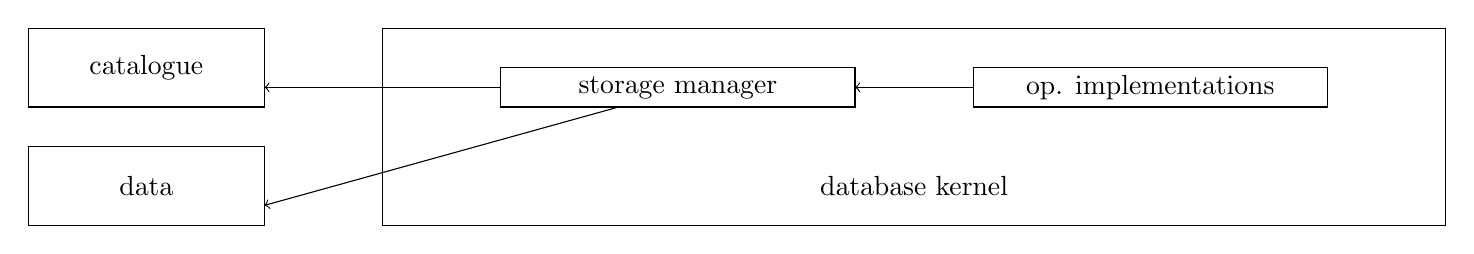
\begin{tikzpicture}[x=1.5cm, y=0.5cm]
                        \draw
                        (0, 0) -- (9, 0) -- (9, -5) -- (0, -5) -- cycle
                        (1, -1) -- (4, -1) -- (4, -2) -- (1, -2) -- cycle
                        (5, -1) -- (8, -1) -- (8, -2) -- (5, -2) -- cycle
                        (-3, 0) -- (-1, 0) -- (-1, -2) -- (-3, -2) -- cycle
                        (-3, -3) -- (-1, -3) -- (-1, -5) -- (-3, -5) -- cycle;

                        \node at (2.5, -1.5) {storage manager};
                        \node at (6.5, -1.5) {op. implementations};
                        \node at (-2, -1) {catalogue};
                        \node at (-2, -4) {data};
                        \node at (4.5, -4) {database kernel};
                        \draw
                        (5, -1.5) edge[->] (4, -1.5)
                        (1, -1.5) edge[->] (-1, -1.5)
                        (2, -2) edge[->] (-1, -4.5);
                    \end{tikzpicture}
                \end{center}
                The DBMS architecture is as follows;
                \begin{center}
                    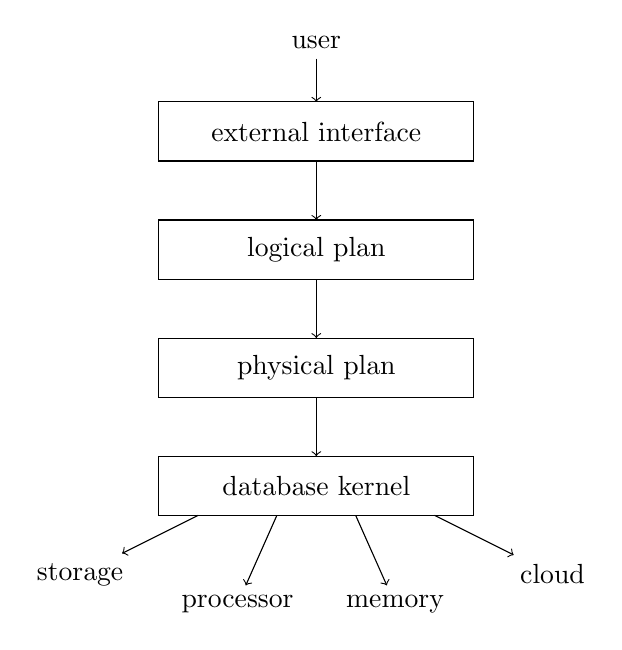
\begin{tikzpicture}[y=0.75cm]
                        \node (u) at (2, 1) {user};
                        \node at (2, -0.5) {external interface};
                        \node at (2, -2.5) {logical plan};
                        \node at (2, -4.5) {physical plan};
                        \node at (2, -6.5) {database kernel};
                        \draw (0, 0) -- (4, 0) -- (4, -1) -- (0, -1) -- cycle;
                        \draw (0, -2) -- (4, -2) -- (4, -3) -- (0, -3) -- cycle;
                        \draw (0, -4) -- (4, -4) -- (4, -5) -- (0, -5) -- cycle;
                        \draw (0, -6) -- (4, -6) -- (4, -7) -- (0, -7) -- cycle;
                        \node (storage) at (-1, -8) {storage};
                        \node (cpu) at (1, -8.5) {processor};
                        \node (mem) at (3, -8.5) {memory};
                        \node (cloud) at (5, -8) {cloud};
                        \draw
                        (u) edge[->] (2, 0)
                        (2, -1) edge[->] (2, -2)
                        (2, -3) edge[->] (2, -4)
                        (2, -5) edge[->] (2, -6)
                        (0.5, -7) edge[->] (storage)
                        (1.5, -7) edge[->] (cpu)
                        (2.5, -7) edge[->] (mem)
                        (3.5, -7) edge[->] (cloud);
                    \end{tikzpicture}
                \end{center}
                The kernel interface, in C++, would look like the following;
                \begin{lstlisting}
                    class StorageManager;
                    class OperatorImplementations;

                    // just provides an interface to the above
                    class DatabaseKernel {
                        StorageManager& getStorageManager();
                        OperatorImplementations& getOperatorImplementations();
                    }
                \end{lstlisting}
            \subsubsection*{Storage}
                The first operation every database needs to support inserting new tuples.
                These inserts are usually not optimised (generally) - they arrive at the storage layer as intact tuples.
                Consider the following example, in SQL;
                \begin{lstlisting}
                    CREATE TABLE Employee (
                        id int,
                        name varchar,
                        salary int,
                        joiningDate int
                    );

                    INSERT INTO Employee VALUES(1, 'james', 100000, 43429342);
                    SELECT * FROM Employee WHERE id=1;
                    DELETE FROM Employee WHERE name='james';
                \end{lstlisting}
                The equivalent in C++ would be as follows;
                \begin{lstlisting}
                    StorageManager().getTable("Employee").insert({1, "james", 100000, 43429342});
                    StorageManager().getTable("Employee").findTuplesWithAttributeValue(id, 4);
                    StorageManager().getTable("Employee").deleteTuplesWithAttributeValue(name, "james");
                \end{lstlisting}
                The storage manager interface would be as follows;
                \begin{lstlisting}
                    struct Table;
                    class StorageManager {
                        map<string, Table> catalogue;

                        public:
                            Table& getTable(string name) {return catalogue[name]; };
                    };
                \end{lstlisting}
                In order to store tuples, we need to decide where and how we store data.
                Generally, for where we store it, we mainly consider disk or memory.
                The way we store data can vary from being sorted, compressed, RLE-encoded, etc.
                A simple table interface could be as follows;
                \begin{lstlisting}
                    struct Table {
                        using AttributeValue = variant<int, float, string>;
                        using Tuple = vector<AttributeValue>;

                        void insert(Tuple) {};
                        vector<Tuple> findTuplesWithAttributeValue(int attributePosition, AttributeValue value) {};
                        void deleteTuplesWithAttributeValue(int attributePosition, AttributeValue value) {};
                    };
                \end{lstlisting}
                There is a fundamental mismatch in storing tuples; relations are two-dimensional, whereas memory is one-dimensional, therefore tuples need to be linearized in one of the two mainstream strategies;
                \begin{itemize}
                    \itemsep0em
                    \item \textbf{The N-ary Storage Model} (NSM)
                        \subitem
                            In this model, the entries added are stored one after the other, in a one-to-one mapping onto memory.
                            This is also referred to as a \textbf{row store}.
                            An example of this is as follows;
                            \begin{lstlisting}
                                struct NSMTable : public Table {

                                    // not the tuple exposed to the outside
                                    struct InternalTuple {
                                        Tuple actualTuple;
                                        bool deleted = false;
                                        InternalTuple(Tuple t) : actualTuple(t) {};
                                    }
                                    vector<InternalTuple> data;

                                    void insert(Tuple);
                                    vector<Tuple> findTuplesWithAttributeValue(int attributePosition, AttributeValue value) {};
                                    void deleteTuplesWithAttributeValue(int attributePosition, AttributeValue value) {};
                                };

                                // declared as member of a class (just append to a vector)
                                void NSMTable::insert(Tuple t) { data.push_back(t); }

                                vector<Table::Tuple> NSMTable::findTuplesWithAttributeValue(int attributePosition, AttributeValue value) {
                                    vector<Tuple> result;
                                    for (size_t i = 0; i < data.size(); i++) {
                                        if (data[i].actualTuple[attributePosition] == value && !data[i].deleted) {
                                            result.push_back(data[i].actualTuple);
                                        }
                                    }
                                    return result;
                                }

                                // we don't want to move everything therefore we just mark them as deleted
                                void NSMTable::deleteTuplesWithAttributeValue(int attributePosition, AttributeValue value) {
                                    for (size_t i = 0; i < data.size(); i++) {
                                        if (data[i].actualTuple[attributePosition] == value) {
                                            data[i].deleted = true;
                                        }
                                    }
                                }
                            \end{lstlisting}
                            However, this may not always be a good idea, as operations will require us going over the entire vector.
                            Recall that we are assuming everything is in memory, however locality still matters (since the data may be further apart depending on the size of the tuple).
                            \medskip

                            Memory is organised in \textbf{cache lines} (usually 64 bytes in size).
                            When a core needs something, it asks L1, L2, and L3 cache first, before going to memory, and retrieves the entire cache line that the data resides on (and cache into L1 cache).
                            If we then access something on the same cache line, then the access is almost free (in terms of time).
                            More tuples will therefore fit on a single cache line if they are smaller.
                            Cache lines can also be referred to as \textbf{blocks} or \textbf{pages}.
                            \medskip

                            N-ary storage works well in inserting a new tuple, when we are inserting a tuple onto the same cache line.
                            It also works well when we want to retrieve a tuple by its index.
                            On the other hand, it's suboptimal when we want to check every row, which in the worst case will be across different cache lines.
                    \item \textbf{Decomposed Storage Model} (DSM)
                        \subitem
                            On the other hand, in this model, entries are stored with the columns one after the other.
                            This is also referred to as \textbf{column store}.
                            An example of this implementation is as follows;
                            \begin{lstlisting}
                                struct DSMTable : public Table {
                                    using Column = vector<AttributeValue>;
                                    vector<Column> data;
                                    vector<bool> deleteMarkers;

                                    void insert(Tuple);
                                    vector<Tuple> findTuplesWithAttributeValue(int attributePosition, AttributeValue value) {};
                                    void deleteTuplesWithAttributeValue(int attributePosition, AttributeValue value) {};
                                };

                                // inserts cause tuple decomposition
                                void DSMTable::insert(Tuple tuple) {
                                    for (int i = 0; i < tuple.size(); i++) {
                                        data[i].push_back(tuple[i]);
                                    }
                                }

                                // find requires tuple reconstruction
                                vector<Table::Tuple> DSMTable::findTuplesWithAttributeValue(int attributePosition, AttributeValue value) {
                                    vector<Tuple> result;
                                    for (size_t i = 0; i < data[attributePosition].size(); i++) {
                                        if (data[attributePosition][i] == value && !deleteMarkers[i]) {
                                            Tuple reconstructedTuple;
                                            for (int column = 0; column < data.size(); column++) {
                                                reconstructedTuple.push_back(data[column][i]);
                                            }
                                            result.push_back(reconstructedTuple);
                                        }
                                    }
                                    return result;
                                }

                                void DSMTable::deleteTuplesWithAttributeValue(int attributePosition, AttributeValue value) {
                                    for (size_t i = 0; i < data.size(); i++) {
                                        if (data[attributePosition][i] == value) {
                                            deleteMarkers[i] = true;
                                        }
                                    }
                                }
                            \end{lstlisting}
                            Decomposed storage works well in the case when we are iterating over one column of a tuple.
                            However, if these entries are one after the other, there is perfect data locality, which minimises the number of cache lines we need.
                            On the other hand, insertion is suboptimal as we need to spread a tuple over memory.
                            Similarly, accessing a single tuple, even when we know where it is in memory is suboptimal, as the tuple will need to be reconstructed.
                    \item Hybrid Delta / Main Storage
                        \begin{lstlisting}
                            struct HybridTable : public Table {
                                DSMTable main; // every tuple will eventually end up here
                                NSMTable delta; // will be inserted here then merged into main

                                void insert(Tuple);
                                vector<Tuple> findTuplesWithAttributeValue(int attributePosition, AttributeValue value) {};
                                void deleteTuplesWithAttributeValue(int attributePosition, AttributeValue value) {};
                                void merge();
                            };

                            void HybridTable::insert(Tuple t) {
                                delta.insert(t);
                            }

                            vector<Table::Tuple> HybridTable::findTuplesWithAttributeValue(int attributePosition, AttributeValue value) {
                                vector<Tuple> results = main.findTuplesWithAttributeValue(attributePosition, value);
                                vector<Tuple> fromDelta = delta.findTuplesWithAttributeValue(attributePosition, value);
                                results.insert(results.end(), fromDelta.begin(), fromDelta.end());
                                return results;
                            }

                            void HybridTable::deleteTuplesWithAttributeValue(int attributePosition, AttributeValue value) {
                                main.deleteTuplesWithAttributeValue(attributePosition, value);
                                delta.deleteTuplesWithAttributeValue(attributePosition, value);
                            }

                            void HybridTable::merge() {
                                for (auto i = 0u; i < delta.data.size(); i++) {
                                    // these two operations need to atomic (otherwise we can return the same tuple multiple times)
                                    main.insert(delta.data[i].actualTuple);
                                    delta.data[i].deleted = true;
                                }
                            }
                        \end{lstlisting}
                \end{itemize}
                In conclusion, \textbf{DSM} works well fro scan-heavy queries (accessing a lot of tuples but few columns).
                This is common in analytical processing, and analytics mostly operate on historical data.
                On the other hand \textbf{NSM} works well for lookups and inserts.
                This is more common in transactional processing (inserting sales item, looking up products, etc).
                Transactions mostly operate on recent data.
                Hybrid exploits the aforementioned workloads, but it needs regular migrations (~merge()~) which may need to lock the database.
            \subsubsection*{Catalogue}
                The catalogue stores metadata.
                The idea is that real-life data follows patterns, which if recognised and exploited, can lead to more efficiency.
                However metadata will need to be stored and maintained.
                Examples of metadata can be type, min / max values (if data is requested outside a range we know it doesn't exist), histograms, etc.
                Two simple ones are \textbf{sortedness} and \textbf{denseness}.
                Consider the following example, which is a common pattern (as the first column is often IDs);
                \begin{lstlisting}
                    class Table {
                        vector<Tuple> storage;
                        bool firstColumnIsSorted = true;
                        bool firstColumnIsDense = true;

                        public:
                            void insert(Tuple t) {
                                if (storage.size() > 0) {
                                    firstColumnIsSorted &= (t[0] >= storage.back()[0]);
                                    firstColumnIsDense &= (t[0] == storage.back()[0] + 1);
                                }
                                storage.push_back(t);
                            }

                            vector<Tuple> findTuplesWithAttributeValue(int attribute, AttributeValue value) {
                                if (attribute == 0 && firstColumnIsDense) {
                                    return { data[value - storage.front()[0]] };
                                } else if (attribute == 0 && firstColumnIsSorted) {
                                    if (binary_search(data, attribute, value)[0] == value) {
                                        return { binary_search(data, attribute, value) };
                                    }
                                }
                                ... // same scan as before
                            }

                            // we can also exploit the fact that order of rows doesn't matter, and therefore we can reorganise
                            void analyse() {
                                // this sort can be expensive (and therefore should be run regularly but not always)
                                sort(storage.begin(), storage.end(), [](auto l, auto r) { return l[0] < r[0] });
                                firstColumnIsSorted = true;
                                firstColumnIsDense = true;
                                for (size_t = 1; i < storage.size(); i++) {
                                    firstColumnIsDense &= storage[i][0] == storage[i - 1][0] + 1;
                                }
                            }
                    }
                \end{lstlisting}
            \subsubsection*{Variable Length Data}
                It's important to note that strings tend to have different lengths.
                However, we'd like to maintain fixed tuple sizes, as it allows for random access to tuples by their position.
                We can either overallocate space for ~varchars~ (for example, some system require a size parameter for maximum length), or we can store them out of place.
                Overallocating leads to strings under the maximum length being padded with some sort of terminator.
                This is good for locality and is simple to implement, however it's very wasteful for space (especially if they are too generous with lengths).
                \medskip

                On the other hand, out of place storage now contain an index into a dictionary, which contains the string (all null terminated).
                However, retrieving a value will need an access to obtain the index and another to get the actual value (which has poor locality).
                While this is better for space (and is what most programming languages do), it's also complicated (and causes difficult garbage-collection).
                This gives an optimisation (\textbf{dictionary compression}) however - if we find a string that has already been used when we insert, we can use the address of the existing value for the insert.
            \subsubsection*{Data Storage on Disk}
                Disks are different from main memory in a number of ways;
                \begin{itemize}
                    \itemsep0em
                    \item \textbf{larger pages} \hfill kilobytes compared to bytes
                    \item \textbf{higher latency} \hfill milliseconds compared to nanoseconds
                    \item \textbf{lower throughput} \hfill hundreds of megabytes instead of tens of gigabytes per second
                        \subitem this is why we consider DBMSs as I/O bound
                    \item \textbf{OS gets in the way} \hfill filesize can be limited, therefore DMBS need to map files and offsets
                \end{itemize}
                Our goals also change slightly; disks now dominate cost, and therefore complicated I/O management strategies can pay off.
                Due to larger pages, each page behaves like a mini-database in the case of N-ary storage.
                The basic kernel now looks like the following (where the catalogue is in memory, but the data is in disk);
                \begin{center}
                    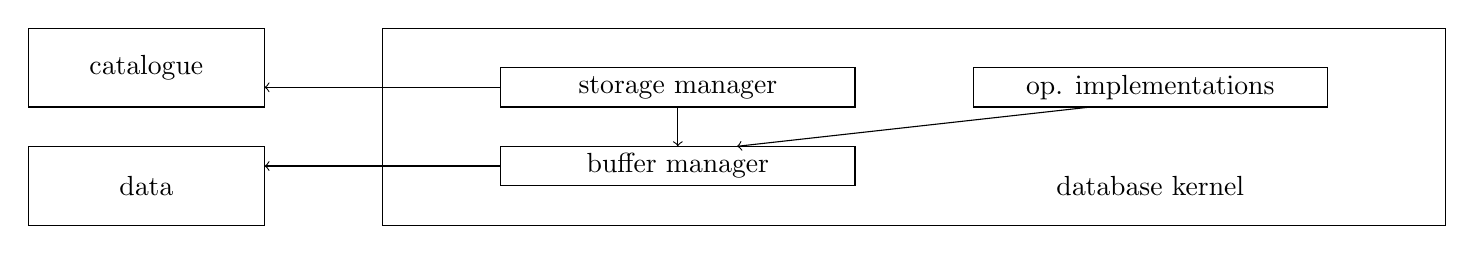
\begin{tikzpicture}[x=1.5cm, y=0.5cm]
                        \draw
                        (0, 0) -- (9, 0) -- (9, -5) -- (0, -5) -- cycle
                        (1, -1) -- (4, -1) -- (4, -2) -- (1, -2) -- cycle
                        (5, -1) -- (8, -1) -- (8, -2) -- (5, -2) -- cycle
                        (1, -3) -- (4, -3) -- (4, -4) -- (1, -4) -- cycle
                        (5, -1) -- (8, -1) -- (8, -2) -- (5, -2) -- cycle
                        (-3, 0) -- (-1, 0) -- (-1, -2) -- (-3, -2) -- cycle
                        (-3, -3) -- (-1, -3) -- (-1, -5) -- (-3, -5) -- cycle;

                        \node at (2.5, -1.5) {storage manager};
                        \node at (2.5, -3.5) {buffer manager};
                        \node at (6.5, -1.5) {op. implementations};
                        \node at (-2, -1) {catalogue};
                        \node at (-2, -4) {data};
                        \node at (6.5, -4) {database kernel};
                        \draw
                        (6, -2) edge[->] (3, -3)
                        (2.5, -2) edge[->] (2.5, -3)
                        (1, -1.5) edge[->] (-1, -1.5)
                        (1, -3.5) edge[->] (-1, -3.5);
                    \end{tikzpicture}
                \end{center}
                The \textbf{buffer manager} manages disk-resident data.
                It maps unstructured files (large 'blobs of bytes') to structured tables for reading and writing.
                Since DBs don't trust OSs, it makes sure files have a fixed size, and it also safely writes data to disk when necessary.
                It also writes in \textbf{open (for writing) pages}.
                An example implementation is as follows;
                \begin{lstlisting}
                    class BufferManager;
                    class Table {
                        BufferManager& bufferManager;
                        string relationName = "Employee";

                        public
                            void insert(Tuple t) {
                                bufferManager.getOpenPageForRelation(relationName).push_back(t);
                                bufferManager.commitOpenPageForRelation(relationName);
                            }

                            vector<Tuple> findTuplesWithAttributeValue(int attribute, AttributeValue value) {
                                vector<Tuple> result;
                                auto pages = bufferManager.getPagesForRelation(relationName);
                                for (size_t i = 0; i < pages.size(); i++) {
                                    auto page = pages[i];
                                    for (size_t i = 0; i < page.size(); i++) {
                                        if (page[i][attribute] == value) {
                                            result.push_back(page[i]);
                                        }
                                    }
                                }
                                return result;
                            }
                    }

                    struct BufferManager {
                        using Tuple = vector<AttributeValue>;
                        using Page = vector<Tuple>;

                        size_t tupleSize;
                        map<string, vector<Tuple>> openPages;
                        map<string, vector<string>> pagesOnDisk; // maps one relation to many pages on disk (filenames)
                        size_t numberOfTuplesPerPage();

                        vector<Tuple>& getOpenPageForRelation(string relationName);
                        void commitOpenPageForRelation(string relationName);
                        vector<Page> getPagesForRelation(string, relationName);
                    }

                    vector<Tuple>& BufferManager::getOpenPageForRelation(string relationName) {
                        return openPages[relationName]; // creates one if needed
                    }

                    void BufferManager::commitOpenPageForRelation(string relationName) {
                        while (openPages[relationName].size() >= numberOfTuplesPerPage(tupleSize)) {
                            vector<Tuple> newPage;

                            // move overflowing tuples to new page
                            while (openPages[relationName].size() > numberOfTuplesPerPage(tupleSize)) {
                                newPage.push_back(openPages[relationName].back());
                                openPages[relationName].pop_back();
                            }

                            pagesOnDisk[relationName].push_back(writeToDisk(openPages[relationName]));
                            openPages[relationName] = newPage; // contains tuples that didn't fit on disk
                        }
                    }

                    vector<vector<Tuple>> BufferManager::getPagesForRelation(string relationName) {
                        vector<vector<Tuple>> result = { openPages[relationName] };
                        for (size_t i = 0; i < pagesOnDisk[relationName].size(); i++) {
                            result.push_back(readFromDisk(pagesOnDisk[relationName][i]));
                        }
                        return result;
                    }
                \end{lstlisting}
                However, we still need to determine ~numberOfTuplesPerPage~;
                \begin{itemize}
                    \itemsep0em
                    \item \textbf{unspanned pages} \hfill pages like mini-databases
                        \subitem
                            The goal of this is simplicity, and good random access performance; we want to find the record with a single page lookup, given a ~tuple\_id~.
                            When we don't have enough space on a page for another tuple, we will write to disk (even when not full) and obtain a new page.
                            However, we can quite easily infer which page a tuple will be on, since we know how many tuples are on each page.
                            This cannot deal with large records (where the size is larger than a page), nor can we have in-page random access if the records are variable size.
                            \begin{lstlisting}
                                const long pageSizeInBytes = 4096;
                                size_t BufferManager::numberOfTuplesPerPage() {
                                    return floor(pageSizeInBytes / tupleSizeInBytes);
                                }

                                // space consumption of a relation of n tuples;
                                ceil(data.size() / mnumberOfTuplesPerPage())
                            \end{lstlisting}
                    \item \textbf{spanned pages} \hfill optimising for space efficiency
                        \subitem
                            On the other hand, the goal here is to minimise space waste and to support large records.
                            Spanned pages can have tuples existing across pages - this is complicated and also hurts random access performance, since we can no longer easily determine where a tuple is.
                            We can calculate the number of pages per relation as follows;
                            \begin{lstlisting}
                                long dataSizeInBytes = tupleSizeInBytes * data.size();
                                long numberOfPagesForTable = ceil(dataSizeInBytes / pageSizeInBytes);
                            \end{lstlisting}
                            However - we cannot determine the number of tuples per page as this is not constant.
                    \item \textbf{slotted pages} \hfill random access for in-place NSM
                        \subitem
                            This is the most complicated method covered, but is also what is used by most systems.
                            This stores tuples in in-place N-ary format, and stores the tuple count in the \textbf{page header} (at the start of the page).
                            Offsets are also stored to every tuple, which are filled in from the \textbf{end} of the page (hence the index of the first tuple is the last item in the page and so on).
                            Offsets need to be typed large enough to address page;
                            \begin{itemize}
                                \itemsep0em
                                \item ~byte~s for pages smaller than 256 bytes
                                \item ~short~s for pages smaller than 65,536 bytes
                                \item ~int~s for pages smaller than 4 gigabytes
                            \end{itemize}
                \end{itemize}
                Some disk-based database systems also keep a dictionary per page, which solves the problem of variable sized records (and allows for duplicate elimination, at the granularity of a single page, as previously mentioned).
                A global dictionary is not used as it will lead to more accesses.
        \subsection*{Lecture 3}
            \subsubsection*{Join}
                The issue with data normalisation (see \textbf{CO130}) is that data ends up scattered across different tables.
                For example, consider the following example tables.
                Notice how a simple application is now split across these 4 tables - but we care more about who ordered what book, rather than the order IDs.
                \begin{center}
                    \hfill
                    \begin{tabular}{ccc}
                        \multicolumn{3}{c}{~Customer~} \\
                        ~ID~ & ~Name~ & ~City~ \\
                        \hline
                        ~1~ & ~james~ & ~London~ \\
                        ~2~ & ~steve~ & ~London~ \\
                        ~3~ & ~kate~ & ~Manchester~ \\
                        \phantom{}
                    \end{tabular}
                    \hfill
                    \begin{tabular}{cc}
                        \multicolumn{2}{c}{~Order~} \\
                        ~ID~ & ~CustomerID~ \\
                        \hline
                        ~1~ & ~1~ \\
                        ~2~ & ~2~ \\
                        ~3~ & ~3~ \\
                        \phantom{}
                    \end{tabular}
                    \hfill
                    \begin{tabular}{cc}
                        \multicolumn{2}{c}{~OrderedItem~} \\
                        ~ID~ & ~CustomerID~ \\
                        \hline
                        ~1~ & ~1~ \\
                        ~1~ & ~2~ \\
                        ~2~ & ~1~ \\
                        ~3~ & ~3~
                    \end{tabular}
                    \hfill
                    \phantom{}
                    \smallskip

                    \hfill
                    \begin{tabular}{ccc}
                        \multicolumn{3}{c}{~Book~} \\
                        ~ID~ & ~Title~ & ~Author~ \\
                        \hline
                        ~1~ & ~Fahrenheit 451~ & ~Ray Bradbury~ \\
                        ~2~ & ~Animal Farm~ & ~George Orwell~ \\
                        ~3~ & ~Distributed Systems~ & ~van Steen \& Tanenbaum~ \\
                        \phantom{}
                    \end{tabular}
                    \hfill
                    \phantom{}
                \end{center}
                Joins are very common not only due to normalisation (with mostly \textbf{Foreign-Key joins}), but also due to the value produced by combining data.
                For example, we can find users that purchase the same product with joins, or finding what advertisements work (seeing which users search for a term within a timeframe after seeing an advert).
                \medskip

                Joins are basically cross products with a selection \textbf{involving both inputs}.
                The variations on joins are based on how tuples without corresponding rows on either input are matched;
                \begin{itemize}
                    \itemsep0em
                    \item \textbf{left join} \hfill ($R \ljoin S$)
                        \subitem
                            This returns all rows in $R$, even if no rows in $S$ match (in this case it fills the columns of $S$ with ~NULL~ values)
                    \item \textbf{right join} \hfill ($R \rjoin S$)
                        \subitem
                            Same as above, but the inverse
                    \item \textbf{full outer join} \hfill ($R \ojoin S$)
                        \subitem
                            Returns every row in $R$ as well as every row in $S$ (even if no rows are matching) - similarly will fill with ~NULL~ values if nothing is matching;
                            $$R \ojoin S \equiv (R \ljoin S) \cup (R \rjoin S)$$
                \end{itemize}
                An example of the matching function is as follows;
                \begin{center}
                    ~SELECT * FROM R JOIN S ON (R.r = S.s)~
                \end{center}
                The matching function for joins does not have to be equality;
                \begin{itemize}
                    \itemsep0em
                    \item \textbf{equi-join} (algorithmically equivalent to intersections) \hfill equality
                    \item \textbf{inequality joins} \hfill inequality constraint (~<~ or ~>~)
                    \item \textbf{anti-join} \hfill ~<>~ or ~!=~
                    \item \textbf{Theta joins} \hfill all other joins (difficult to optimise)
                \end{itemize}
            \subsubsection*{Join Algorithms}
                Some of the join algorithms are as follows;
                \begin{itemize}
                    \itemsep0em
                    \item \textbf{nested loop join}
                        \begin{lstlisting}
                            using Table = vector<vector<int>>;
                            Table left, right;
                            for (size_t i = 0; i < leftRelationSize; i++) {
                                auto leftInput = left[i];
                                for (size_t j = 0; j < rightRelationSize; j++) {
                                    auto rightInput = right[j];
                                    if (leftInput[leftAttribute] == rightInput[rightAttribute]) {
                                        writeToOutput({leftInput, rightInput});
                                    }
                                }
                            }
                        \end{lstlisting}
                        This is a simple algorithm and is trivial to parallelise (since there are no dependent loop iterations).
                        This also has sequential I/O, which is good for the buffer manager.
                        The effort required however is;
                        $$\Theta(|L| \times |R|) \text{ , reduced to } \Theta\left(\frac{|L| \times |R|}{2}\right) \text{ if uniqueness can be assumed}$$
                    \item \textbf{sort-merge joins}
                        \begin{lstlisting}
                            // this assumes values are unique and sorted
                            auto leftI = 0;
                            auto rightI = 0;
                            // keep iterating until either input is finished
                            while (leftI < leftInputSize && rightI < rightInputSize) {
                                auto leftInput = left[leftI];
                                auto rightInput = right[leftI];
                                if (leftInput[leftAttribute] < rightInput[rightAttribute]) {
                                    leftI++;
                                } else if (rightInput[rightAttribute] > leftInput[leftAttribute]) {
                                    rightI++;
                                } else {
                                    writeToOutput({leftInput, rightInput});
                                    rightI++;
                                    leftI++;
                                }
                            }
                        \end{lstlisting}
                        The idea of this is that we first sort both inputs and have cursors starting at the start of each input.
                        If the value at the left pointer is smaller than the value at the right pointer, we increment the left pointer (and vice versa).
                        If it's the same, then we can output a match.
                        \medskip

                        Assuming (without loss of generality) the value of on the left is less than the value on the right.
                        All values after the value on the right are greater than it (due to the sorted nature).
                        Therefore no value after the value on the right can be a join partner to the value on the left, therefore we can advance the cursor on the left.
                        \begin{center}
                            \begin{tikzpicture}[x=1.5cm, y=0.75cm]
                                \node (f) at (0, -3) {5};
                                \node (s) at (3, -2) {7};
                                \draw
                                (0, 0) edge[dashed] (f)
                                (f) edge[dashed, left] node{$>5$} (0, -5)
                                (3, 0) edge[dashed] (s)
                                (s) edge[dashed, right] node{$>7$} (3, -5)
                                (5, 0) edge[->, right] node{merge direction} (5, -5)
                                (f) edge[<->, above] node{comparison} (s);
                            \end{tikzpicture}
                        \end{center}
                        The effort required for this is as follows (the merge must go through each tuple on either side);
                        $$O(\underbrace{|L| \times \log|L|}_{O(~sort~(L))} + \underbrace{|R| + \log|R|}_{O(~sort~(R))} + \underbrace{|L| + |R|}_{O(~merge~)})$$
                        This has sequential I/O in the merge phase, however it is tricky to parallelise.
                        This also works for inequality joins, but we need to be more careful when advancing the cursors.
                    \item \textbf{hash joins}
                        \begin{lstlisting}
                            vector<optional<vector<int>>> hashTable; // optional since slots can be empty
                            int hash(int);
                            int nextSlot(int);

                            for (size_t i = 0; i < buildSide.size(); i++) {
                                auto buildInput = buildSide[i];
                                auto hashValue = hash(buildInput[buildAttribute]);

                                // avoid overwriting a value
                                while (hashTable[hashValue].hasValue) {
                                    hashValue = nextSlot(hashValue);
                                }
                                hashTable[hashValue] = buildInput;
                            }

                            for (size_t i = 0; i < probeSide.size(); i++) {
                                auto probeInput = probeSide[i];
                                auto hashValue = hash(probeInput[probeAttribute]);
                                while (hashTable[hashValue].hasValue && hashTable[hashValue].value[buildAttribute] != probeInput[probeAttribute]) {
                                    hashValue = nextSlot(hashValue);
                                }
                                if (hashTable[hashValue].value[buildAttribute] == probeInput[probeAttribute]) {
                                    writeToOutput({hashTable[hashValue].value, probeInput})
                                }
                            }
                        \end{lstlisting}
                        We need to first distinguish the \textbf{build-side} (side buffered in the hashtable) and \textbf{probe-side} (side used to look up tuples in the hashtable).
                        \medskip

                        For this, we need to establish some requirements on the hash function.
                        The requirements is that it is pure (and has no state), and need to know the output domain (the range of generated values) in order to allocate the size.
                        It's also ideal to have a contiguous output domain (without holes) and a uniform distribution (where all values are equally likely for consistent performance).
                        Some common examples are;
                        \begin{itemize}
                            \itemsep0em
                            \item \textbf{MD5}
                            \item \textbf{Modulo-Division} \hfill simplest (but input skew leads to output skew)
                            \item \textbf{MurmurHash} \hfill one of fastest, decent hash-functions
                            \item \textbf{CRC32} \hfill also has input skew issue, but has hardware support
                        \end{itemize}
                        Furthermore, we need to handle conflicts on hash collision.
                        This needs to have some locality (if there is too much locality, there can be issues when inserting a lot of data into the same slot).
                        Additionally, it needs to have no holes (we want to probe all slots to avoid memory waste).
                        Some approaches are as follows;
                        \begin{itemize}
                            \itemsep0em
                            \item \textbf{linear probing}
                                \subitem
                                    When a slot is filled, try the next one and continue doing so until a free slot is found - wrapping around to the start at the end of the buffer.
                                    This approach is simple and has great access locality.
                                    However it can lead to long probe-chains for adversarial input data (if we have input locality).
                            \item \textbf{quadratic probing}
                                \subitem
                                    This is similar to the above strategy, but we instead double the distance from the initial slot each time, first checking one that is a distance of 1 away, then 2, then 4, and so on, also wrapping at the end of the buffer.
                                    This is also simple, but only has good locality for the first few probes (and gets much worse).
                                    The first few probes are also likely to cause conflicts.
                            \item \textbf{rehashing}
                                \subitem
                                    We want to distribute probes uniformly, which can cause poor access locality but reduces conflicts.
                                    To do so, we can just use the hash function again.
                                    However, to ensure all slots are probed, we need to consider \textbf{cyclic groups}.
                        \end{itemize}
                        An example of this applied, with \textbf{modulo hashing} (with a constant factor of 10 for simplicity) and \textbf{linear probing} is as follows;
                        \begin{lstlisting}
                            int hash(int v) { return v % 10; }
                            int probe(int v) { return (v + 1) % 10; }

                            buildSide = {1, 2, 7, 8, 12, 16, 17};
                        \end{lstlisting}
                        With this, we'd end up with the following slots in the hash table (~-~ denotes unused);
                        \begin{center}
                            ~(index 0) => [-, 1, 2, 12, -, -, 16, 7, 8, 17] <= (index 9)~
                        \end{center}
                        Hash joins give us sequential I/O on inputs but pseudo-random access to the hash-table during build and probe.
                        It's parallelisable over the values on the probe side, but parallelising the build is difficult.
                        The effort required is;
                        $$\Theta(|~build~| + |~probe~|) \text{ (best case) and } O(|~build~| \times |~probe~|) \text{ (worst case)}$$
                        However, it's also important to consider that we typically want to store more than a single value, and often we may not have the uniqueness guarantee.
                        Good hashing is still expensive and requires lots of CPU cycles (more expensive than multiple data accesses).
                        Slots are often also allocated in buckets, allow for more than one tuple per slot.
                        It's roughly equivalent to rounding every hash value down to a multiple of the bucket size.
                        Sometimes buckets are implemented as linked lists (\textbf{bucket-chaining}, \textbf{open addressing}) which is a bad idea for lookup performance.
                        Hashtables are also arrays, which occupy space (typically overallocated by a factor of two to reduce long probe chains).
                        They are also probed randomly in the probe phase, ideally we want to keep the hash table in memory / cache, but not to disk.
                        \textbf{For this class}, if the hashtable doesn't fit, \textbf{every access has a constant penalty}.
                        Generally we use hash joins when one relation is much smaller than the other.
                \end{itemize}
            \subsubsection*{Partitioning}
                We have the fundamental premise that sequential access is much cheaper than random access, and the difference grows with the page size.
                If we assume a random value access cost $c$, the sequential value access cost is;
                $$\frac{c}{\text{pagesize}_\text{OS}}$$
                Assuming the hashtable doesn't fit in the page / cache, we will use the cost $c$ quite frequently, and therefore the extra pass for partitioning, which is mostly sequential access might be worth doing.
                We can visualise thrashing as follows;
                \begin{center}
                    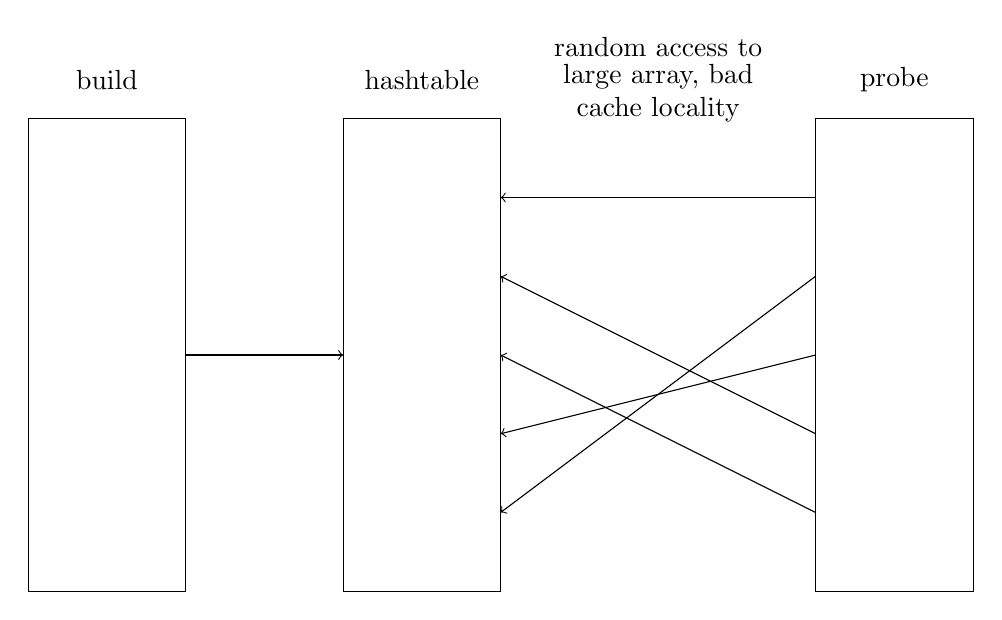
\begin{tikzpicture}
                        \node at (1, 0.5) {build};
                        \node at (5, 0.5) {hashtable};
                        \node at (11, 0.5) {probe};
                        \node at (8, 0.5) {\shortstack{random access to\\large array, bad\\cache locality}};
                        \draw
                        (2, -3) edge[->] (4, -3)
                        (0, 0) -- (2, 0) -- (2, -6) -- (0, -6) -- cycle
                        (4, 0) -- (6, 0) -- (6, -6) -- (4, -6) -- cycle
                        (10, 0) -- (12, 0) -- (12, -6) -- (10, -6) -- cycle;
                        \draw
                        (10, -1) edge[->] (6, -1)
                        (10, -2) edge[->] (6, -5)
                        (10, -3) edge[->] (6, -4)
                        (10, -4) edge[->] (6, -2)
                        (10, -5) edge[->] (6, -3);
                    \end{tikzpicture}
                \end{center}
                On the other hand, by using a partitioning function (which typically has a small range to fit stuff into memory);
                \begin{center}
                    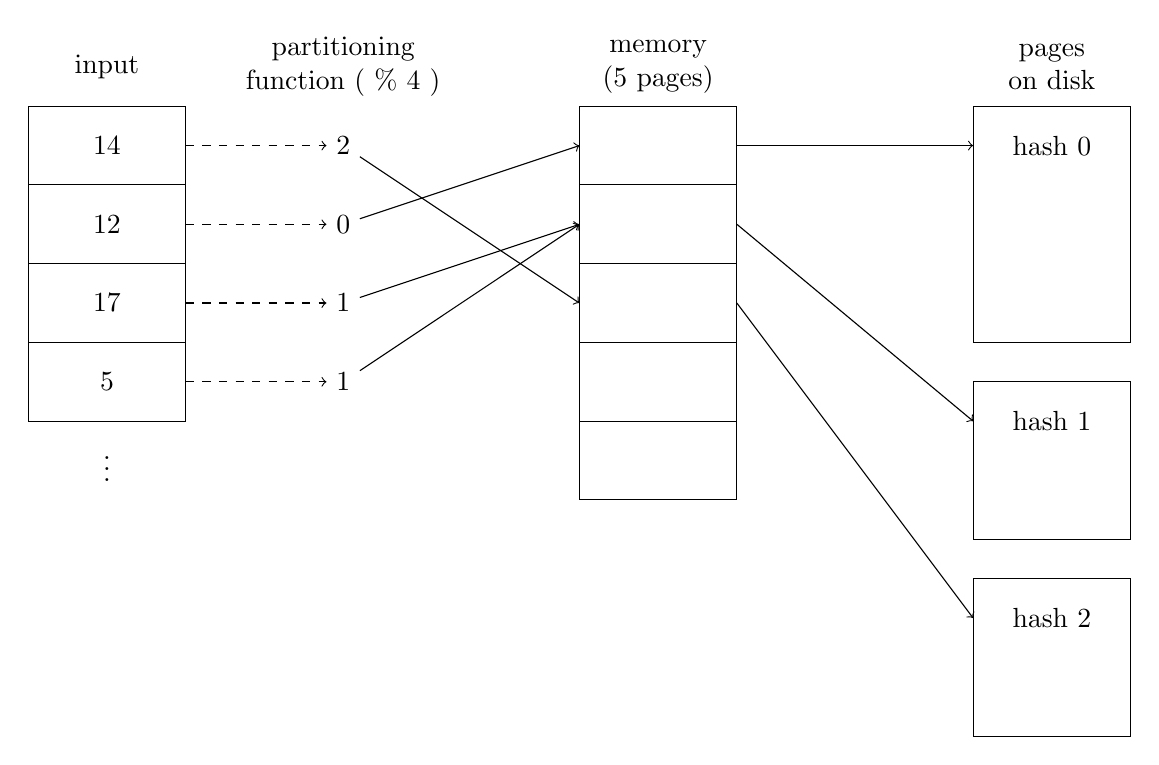
\begin{tikzpicture}
                        \node at (1, 0.5) {input};
                        \node at (4, 0.5) {\shortstack{partitioning\\function (~\% 4~)}};
                        \node at (8, 0.5) {\shortstack{memory\\(5 pages)}};
                        \node at (13, 0.5) {\shortstack{pages\\on disk}};
                        \node at (1, -0.5) {14};
                        \node at (1, -1.5) {12};
                        \node at (1, -2.5) {17};
                        \node at (1, -3.5) {5};
                        \node (p0) at (4, -0.5) {2};
                        \node (p1) at (4, -1.5) {0};
                        \node (p2) at (4, -2.5) {1};
                        \node (p3) at (4, -3.5) {1};
                        \node at (13, -0.5) {hash 0};
                        \node at (13, -4) {hash 1};
                        \node at (13, -6.5) {hash 2};
                        \node at (1, -4.5) {$\vdots$};
                        \draw
                        (2, -0.5) edge[dashed, ->] (p0)
                        (p0) edge[->] (7, -2.5)
                        (p1) edge[->] (7, -0.5)
                        (p2) edge[->] (7, -1.5)
                        (p3) edge[->] (7, -1.5)
                        (2, -1.5) edge[dashed, ->] (p1)
                        (2, -2.5) edge[dashed, ->] (p2)
                        (2, -3.5) edge[dashed, ->] (p3)
                        (9, -0.5) edge[->] (12, -0.5)
                        (9, -1.5) edge[->] (12, -4)
                        (9, -2.5) edge[->] (12, -6.5);
                        \draw
                        (0, -1) -- (2, -1)
                        (0, -2) -- (2, -2)
                        (0, -3) -- (2, -3)
                        (0, 0) -- (2, 0) -- (2, -4) -- (0, -4) -- cycle;
                        \draw
                        (7, -1) -- (9, -1)
                        (7, -2) -- (9, -2)
                        (7, -3) -- (9, -3)
                        (7, -4) -- (9, -4)
                        (7, 0) -- (9, 0) -- (9, -5) -- (7, -5) -- cycle;
                        \draw
                        (12, 0) -- (14, 0) -- (14, -3) -- (12, -3) -- cycle
                        (12, -3.5) -- (14, -3.5) -- (14, -5.5) -- (12, -5.5) -- cycle
                        (12, -6) -- (14, -6) -- (14, -8) -- (12, -8) -- cycle;
                    \end{tikzpicture}
                \end{center}
                The write from input to memory is done for every tuple, but the write from memory to the pages on the disk is only done when the page is \textbf{filled}, which doesn't waste bandwidth (and also lowers the number of $c$s we use).
                As such, the probing becomes more involved, we first partition the probe in the same way, and we then only look at the partitioned hashtables, which gives us localised random access.
                \medskip

                Another benefit of partitioning is that we can now parallelise the processing of each of the smaller joins, since we know they are disjoint.
            \subsubsection*{Indexing}
                We should note that these algorithms are done in phases (build / probe and sort / merge).
                Typically the first phase, build or sort, is independent of the query phase, and can be done before any data is requested (such as when it is first loaded in).
                This is called indexing.
                \medskip

                An index is a secondary storage, which is about replicating data.
                The replication is controlled by the DBMS, which means they can be created and destroyed without breaking the system.
                These replicas are semantically invisible to the user (doesn't change results).
                On the other hand, these replicas occupy space and need to be maintained under updates.
                \medskip

                A primary index is used to store the tuples of a table, not a table, and therefore only one of these can be used per table.
                On the other hand, a secondary index stores pointers to the tuple of a table, hence we can have many of these in a table.
                \medskip

                In SQL, an index can be created and destroyed as follows (however, it's unclear what type of index is created, nor do we have control over parameters);
                \begin{lstlisting}
                    CREATE INDEX index_name ON table_name (column1, column2, ...);
                    DROP INDEX index_name;
                \end{lstlisting}
                Some examples are as follows;
                \begin{itemize}
                    \itemsep0em
                    \item \textbf{Hash-Indexing}
                        \subitem
                            The first step of a hash-join was building a hash-table, instead the hash-index is the same but persistent.
                            In an unclustered hash-index, there is hash table which stores the key and position, and in the relation it is ordered by the position (and contains the actual data).
                            \medskip

                            The \textbf{ephemeral} hashtables we built for hash-joins were temporary, and we assume that no new tuples are added during the evaluation of the query, and we'd also know a rough amount of tuples that would end up in the table.
                            However, all of this changes if the hash-table is persistent.
                            Since persistent tables may grow arbitrarily large, we need to overallocate by a lot.
                            If the fill-factor grows beyond $x$ percent, we need to rebuild it with a larger overallocation - this can be expensive (and leads to load spikes on the inserts causing rebuilds).
                            Similar, deletion can also be problematic.
                            \medskip

                            Previously, we used empty slots to mark an end of a probe-chain.
                            However, a value must remain if something is deleted - we can either leave the value and mark it as deleted, or put the last value in the probe chain in the position.
                            A deletion strategy (to delete key ~k~) is as follows;
                            \begin{itemize}
                                \itemsep0em
                                \item hash ~k~, find ~k~, and keep a pointer to ~k~
                                \item continue probing until the end of the probe chain is found
                                \item if the value at the end of the chain has the same hash as ~k~, move it into ~k~'s slot
                                \item otherwise mark ~k~ as deleted (we can then fill this slot with the next value that hashes into the probe chain)
                            \end{itemize}
                            An example is as follows.
                            Note that 14 has the same hash as 23 (under modulo 9), but 14 has a different hash to 17.
                            \begin{center}
                                \begin{tabular}{c|ccc|c}
                                    \multicolumn{5}{c}{before} \\
                                    \hline
                                    key & \multicolumn{3}{c|}{non-key} & deleted \\
                                    \hline
                                    9 & 16 & 9 & 34 & \\
                                    27 & 5 & 61 & 45 & \\
                                    12 & 12 & 78 & 1 & \\
                                    & & & & \\
                                    23 & 84 & 17 & 69 & \\
                                    5 & 45 & 71 & 20 & \\
                                    17 & 9 & 42 & 83 & \\
                                    14 & 21 & 55 & 2 & \\
                                    & & & &
                                \end{tabular}
                                \hfill
                                \begin{tabular}{c|ccc|c}
                                    \multicolumn{5}{c}{after delete 23} \\
                                    \hline
                                    key & \multicolumn{3}{c|}{non-key} & deleted \\
                                    \hline
                                    9 & 16 & 9 & 34 & \\
                                    27 & 5 & 61 & 45 & \\
                                    12 & 12 & 78 & 1 & \\
                                    & & & & \\
                                    14 & 21 & 55 & 2 & \\
                                    5 & 45 & 71 & 20 & \\
                                    17 & 9 & 42 & 83 & \\
                                    & & & & \\
                                    & & & &
                                \end{tabular}
                                \hfill
                                \begin{tabular}{c|ccc|c}
                                    \multicolumn{5}{c}{after delete 14} \\
                                    \hline
                                    key & \multicolumn{3}{c|}{non-key} & deleted \\
                                    \hline
                                    9 & 16 & 9 & 34 & \\
                                    27 & 5 & 61 & 45 & \\
                                    12 & 12 & 78 & 1 & \\
                                    & & & & \\
                                    14 & 21 & 55 & 2 & $\times$ \\
                                    5 & 45 & 71 & 20 & \\
                                    17 & 9 & 42 & 83 & \\
                                    & & & & \\
                                    & & & &
                                \end{tabular}
                            \end{center}
                            Similar to hash-joins, persistent hash-tables are good for hash-joins and aggregations (assuming they are built on the join / aggregation key columns).
                            They also reduce the number of candidates for equality selections, but don't help on much else.
                    \item \textbf{Bitmap-Index}
                        \subitem
                            It's first important to establish a \textbf{bitvector} is a sequence of 1-bit values indicating a boolean condition holding for the elements of a sequence of values.
                            However, it's important to note that CPUs don't work with individual bits but rather words (let us assume 8 bit words, although in reality it's at least 32 bits);
                            \begin{align*}
                                BV_{== 7}([4, 7, 11, 7, 7, 11, 4, 7]) & = [0, 1, 0, 1, 1, 0, 0, 1] \\
                                & = 128 \cdot 0 + 64 \cdot 1 + 32 \cdot 0 + 16 \cdot 1 + 8 \cdot 1 + 4 \cdot 0 + 2 \cdot 0 + 1 \cdot 1 \\
                                & = 89
                            \end{align*}
                            Bitmap indices are a collection of bitvectors on a column (one for each distinct value in that column).
                            This is useful if there are few distinct values and these bitvectors are disjoint.
                            \begin{center}
                                \begin{tabular}{c|ccc}
                                    column & \multicolumn{3}{c}{bitmap index} \\
                                    & ~==5~ & ~==3~ & ~==9~ \\
                                    \hline
                                    5 & 1 & 0 & 0 \\
                                    3 & 0 & 1 & 0 \\
                                    9 & 0 & 0 & 1 \\
                                    9 & 0 & 0 & 1 \\
                                    9 & 0 & 0 & 1 \\
                                    5 & 1 & 0 & 0 \\
                                    3 & 0 & 1 & 0 \\
                                    9 & 0 & 0 & 1
                                \end{tabular}
                            \end{center}
                            An implementation of this is as follows;
                            \begin{lstlisting}
                                unsigned char** bitmaps;
                                void scanBitmap(byte* column, size_t inputSize, byte value) {

                                    // finds specific bitmap for a certain value
                                    unsigned char* scannedBitmap = bitmapForValue(bitmaps, value);

                                    // iterate over bytes in bitmap
                                    for (size_t i = 0; i < inputSize / 8; i++) {
                                        // skip if none of the values are set
                                        if (scannedBitmap[i] != 0) {
                                            unsigned char bitmapMask = 128; // binary 10000000
                                            for (size_t j = 0; j < 8; j++) {
                                                if ((bitmapMask & scannedBitmap[i]) && column[i * 8 + j] == value) {
                                                    writeOutput(column[i * 8 + j]);
                                                }
                                                bitmapMask >>= 1;
                                            }
                                        }
                                    }
                                }
                            \end{lstlisting}
                            This is useful as it reduces the bandwidth need for scanning a column, in the order of the size of the type of the column in bits (instead of loading a 32 bit value, we can just check 1 bit).
                            Predicates can now also be combined using logical operators on the bitvectors.
                            Additionally, arbitrary boolean conditions (such as ranges) can be indexed by some systems.
                            \medskip

                            Binned bitmaps uses the idea of having $n$ bitvectors, each with a predicate covering a different part of the value domain.
                            For example if we assume our column type is a ~byte~, we can have the following three bins;
                            \begin{itemize}
                                \itemsep0em
                                \item bin 1: 0 - 7
                                \item bin 2: 8 - 20
                                \item bin 3: 21 - 255
                            \end{itemize}
                            We need to ensure the conditions span the entire value domain.
                            Also, the index cannot distinguish values in a bin (unless it only contains one value) - it can only produce \textbf{candidates}, some of which may be false positives.
                            \medskip

                            Generally there are two strategies for binning;
                            \begin{itemize}
                                \itemsep0em
                                \item \textbf{equi-width}
                                    \subitem
                                        This is simple to configure - we can calculate our bin-width to be
                                        $$\frac{\max(~column~) - \min(~column~)}{~numberOfBins~}$$
                                        This has limited use when indexing non-uniformly distributed data (since there can be a high frequency of false positives in a highly populated bin).
                                \item \textbf{equi-height}
                                    \subitem
                                        This method is more resilient against non-uniformly distributed data - the false positive rate is value independent.
                                        We want to have the same number of counts per bin.
                                        The construction is more difficult however, as we need to determine quantiles and is usually performed on samples.
                                        If the distribution changes, it will need to be rebinned (which can be expensive).
                            \end{itemize}
                            Additionally, when we are binning, we may encounter many consecutive values which are equal.
                            Each of these consecutive values can be replaced with the value (the Run) as well as the number of tuples (length) - this works very well on high-locality data.
                            For example, we can transform ~[0, 1, 1, 1, 1, 1, 0, 1]~ to ~[(0, 1), (1, 5), (0, 1), (1, 1)]~.
                            However, this will now require a sequential scan, which can be fixed with \textbf{length prefix summing} (which stores the start of the run instead of the length);
                            ~[(0, 3), (1, 3), (0, 1), (1, 1)]~ to ~[(0, 0), (1, 3), (0, 6), (1, 7)]~.
                            If we were to search for a value, we can just do a binary search instead of a sequential scan.
                    \item \textbf{B-Trees}
                        \subitem
                            Databases are typically I/O bound (for disk), therefore we want to minimise page I/O operations.
                            There are also many equality lookups, as well as many updates.
                            Databases use high-fanout trees to minimise page I/Os.
                            We want the node of a tree to ideally be exactly the same size as a page (if we access a page, we might as well get the maximum amount of information out).
                            Generally, a node in a B-Tree contains pairs (pivots) of keys and payloads, as well as child pointers to other nodes between the pairs (as well as before and after).
                            \medskip

                            A B-Tree is defined as follows;
                            \begin{itemize}
                                \itemsep0em
                                \item a \textbf{balanced tree} with out-degree $n$ (every node has $n - 1$ keys)
                                \item the \textbf{root} has at least one element
                                \item each \textbf{non-root node} contains at least $\floor{\frac{n - 1}{2}}$ key / value pairs (at least half full)
                            \end{itemize}
                            Unlike other trees, B-Trees grow towards the root.
                            In order to maintain balance, on an insertion the following steps apply;
                            \begin{itemize}
                                \itemsep0em
                                \item find the correct \textbf{leaf-node} to insert by walking the tree and inserting the value
                                \item if this node overflows (the leaf was already full), split the node in two halves
                                    \begin{itemize}
                                        \itemsep0em
                                        \item take one pivot from the middle of the leaf and move it to the parent node
                                        \item the two newly created nodes will become the left and right children of the pivot
                                    \end{itemize}
                                \item if the parent overflows, repeat the procedure on the parent
                                \item if the parent is root, a new root node is introduced (therefore we add more roots, rather than add leaves)
                            \end{itemize}
                            For deletion, the following steps apply;
                            \begin{itemize}
                                \itemsep0em
                                \item find the value to delete
                                    \begin{itemize}
                                        \itemsep0em
                                        \item delete it if it is in a leaf node
                                        \item otherwise, if it is in an internal node, keep a pointer to it, and replace it with the maximum leaf-node value from the left-child (removing the value from the leaf-node) - all modifications are on the leaf level
                                    \end{itemize}
                                \item if the affected leaf node underflows, we need to rebalance the tree bottom-up
                                    \begin{itemize}
                                        \itemsep0em
                                        \item try to obtain an element from a neighbouring node (to the right), move that up one level and make it the new splitting pivot, and take the old splitting pivot from the parent and put it into the leaf node
                                        \item however, if that fails (the neighbour isn't more than half full), the nodes can be merged and the parent splitting key can be removed
                                        \item if that causes an underflow, keep rebalancing upwards
                                    \end{itemize}
                            \end{itemize}
                            While B-Trees can support ranges, it is complicated and requires going up and down the tree.
                            This causes many node traversals, however node sizes are usually the same as page sizes, therefore traversals translate into page faults (which we want to minimise).
                            Leaf pointers also aren't used, and most of the data lives in leaf nodes, therefore there is some space wasted.
                    \item \textbf{B$^+$-Trees}
                        \subitem
                            The idea of this is to make range scans faster by keeping data only in the leaves, and linking leaf nodes to the next.
                            Inner-node split values are replicas of leaf-node values.
                            There is now more of a distinction between inner nodes and leaf nodes.
                            The child pointers of the inner nodes are to other nodes, whereas the child pointers of leaf nodes (to the left) are now the payloads for a given key, and the right-most child pointer points to the next leaf.
                            As such, the leaf nodes now form a sorted sequence.
                            \medskip

                            The balancing is largely the same as the balancing for regular B-Trees, however the deletion of an inner-node's split values imply a replacement with a new value from the leaf node.
                    \item \textbf{Foreign-Key Index}
                        \subitem
                            In SQL, a foreign key is as follows;
                            ~ALTER TABLE Orders ADD FOREIGN KEY (BookID\_index) REFERENCES Book(ID)~.
                            FK constraints specify that for for every value that occurs in an attribute of a table, there is exactly one value in the PK column of another table.
                            This constraint must be done by the DBMS, on an insertion or update, the DBMS needs to look up the PK value, and instead of storing the value, the DBMS could store a pointer to the referenced PK or tuple.
                            We can think of this as equivalent to a pointer, and we can consider these as pre-calculated joins (which is often used since most joins are PK/FK joins from normalisation).
                            \medskip

                            Generally there are very few downsides - they cause insignificant work under updates, they do not cost much more space, and doesn't take more effort for query optimisation.
                \end{itemize}
        \subsection*{Lecture 4}
            \subsubsection*{Processing Model}
                A processing model is the mechanism used to connect different operators.
                This matters since different storage models are optimised for different bottlenecks, such as data access, CPU, query compilation, etc.
            \subsubsection*{Function Objects}
                These can be referred to in different ways, such as lambdas, function pointers, etc.
                On a higher level, they are pieces of code that are treated like data (basically just pointers to an instruction) - they can be assigned to variables, invoked with arguments, and will return a value.
                \begin{lstlisting}
                    Python: aggregate = lambda v, t : v + t[0]
                    C++:    function<int(int, Tuple)> aggregate = [](int v, Tuple t) {
                              return v + (int)t[0];
                            };
                \end{lstlisting}
            \subsubsection*{Volcano Processing}
                This influential system was built in the 80s, and focused strongly on design practices, with less of a focus on performance.
                It contained components such as the cascades query optimiser, a non-relational physical algebra, and a query processing model.
                This was designed with flexibility, clean design, maintainability, developer productivity, and a fair bit of tunability in mind.
                \medskip

                The operator interface provided is as follows - they are connected using pointers (in our case the ~unique\_ptr~ smart pointer);
                \begin{lstlisting}
                    struct Operator {
                      virtual void open() = 0;
                      virtual optional<Tuple> next() = 0;
                      virtual void close() = 0;
                    }
                \end{lstlisting}
                Looking at the operators;
                \begin{itemize}
                    \itemsep0em
                    \item \textbf{scan} \hfill read a table and return contained tuples one by one
                        \begin{lstlisting}
                            struct Scan : Operator {
                              Table input;
                              size_t nextTupleIndex = 0; // operators are stateful
                              Scan(Table input) : input(input){};
                              void open(){}; // no work to be done at the start
                              optional<Tuple> next() {
                                return nextTupleIndex < input.size()
                                           ? input[nextTupleIndex++]
                                           : {}; // empty value marks end
                              };
                              void close(){};
                            };
                        \end{lstlisting}
                    \item \textbf{projection} \hfill transform one tuple into another using a projection function
                        \begin{lstlisting}
                            struct Project : Operator {
                              using Projection = function<Tuple(Tuple)>;
                              Projection projection;
                              unique_ptr<Operator> child;
                              void open() { child->open(); };
                              optional<Tuple> next() { return projection(child->next()); };
                              void close() { child->close(); };
                            };
                        \end{lstlisting}
                    \item \textbf{selection} \hfill return all tuples satisfying a boolean predicate
                        \begin{lstlisting}
                            struct Select : Operator {
                              using Predicate = function<bool(Tuple)>;
                              unique_ptr<Operator> child;
                              Predicate predicate;

                              Select(unique_ptr<Operator> child, Predicate predicate)
                                  : child(move(child)), predicate(predicate) {};

                              void open() { child->open(); };
                              optional<Tuple> next() {
                                // iterate until matches or cannot find a tuple
                                for (auto candidate = child->next(); candidate.has_value(); candidate = child->next()) {
                                  if (predicate(candidate)) {
                                    return candidate;
                                  }
                                }
                                return {};
                              };
                              void close() { child->close(); };
                            };
                        \end{lstlisting}
                    \item \textbf{union} \hfill return all tuples from one child followed by all tuples from another
                        \begin{lstlisting}
                            struct Union : Operator {
                              unique_ptr<Operator> leftChild;
                              unique_ptr<Operator> rightChild;
                              void open() {
                                leftChild->open();
                                rightChild->open();
                              };
                              optional<Tuple> next() {
                                auto candidate = leftChild->next();
                                return candidate.has_value() ? candidate : rightChild->next();
                              };
                              void close() {
                                leftChild->close();
                                rightChild->close();
                              };
                            };
                        \end{lstlisting}
                    \item \textbf{difference} \hfill return all tuples from the left that are not in the right (buffer right first)
                        \begin{lstlisting}
                            struct Difference : Operator {
                              unique_ptr<Operator> leftChild;
                              unique_ptr<Operator> rightChild;
                              vector<Tuple> bufferedRight;

                              void open() {
                                leftChild->open();
                                rightChild->open();
                                for (auto rightTuple = rightChild->next(); rightTuple.has_value(); rightTuple = rightChild->next()) {
                                  bufferedRight.push_back(rightTuple);
                                }
                              };
                              optional<Tuple> next() {
                                for (auto candidate = leftChild->next(); candidate.has_value(); candidate = leftChild->next()) {
                                  if (find(bufferedRight.begin(), bufferedRight.end(), candidate) == bufferedRight.end()) {
                                    return candidate;
                                  }
                                }
                                return {};
                              };
                              void close() {
                                leftChild->close();
                                rightChild->close();
                              };
                            };
                        \end{lstlisting}
                        Note that this is an example of a \textbf{pipeline breaker}; an operator that produces the first output tuple after \textbf{all} input tuples from one of the sides have been processed.
                    \item \textbf{cross product}
                        \begin{lstlisting}
                            struct Cross : Operator {
                              unique_ptr<Operator> leftChild;
                              unique_ptr<Operator> rightChild;
                              Tuple currentLeftTuple{};
                              vector<Tuple> bufferedRightTuples;
                              size_t currentBufferedRightOffset = 0;

                              void open() {
                                leftChild->open();
                                rightChild->open();
                                currentLeftTuple = leftChild->next();
                              };
                              optional<Tuple> next() {
                                // some processing moved from open() phase to next() phase
                                auto currentRightTuple = rightChild->next();
                                if (currentRightTuple.has_value()) {
                                  bufferedRightTuples.push_back(currentRightTuple);
                                }
                                if (currentBufferedRightOffset == bufferedRightTuples.size()) {
                                  currentBufferedRightOffset = 0;
                                  currentLeftTuple = leftChild->next();
                                }
                                return currentLeftTuple.concat(bufferedRightTuples[currentBufferedRightOffset++]);
                              };
                              void close() {
                                leftChild->close();
                                rightChild->close();
                              };
                            };
                        \end{lstlisting}
                        Since we are able to implement this without breaking the pipeline, the implementation of an operator determines whether an operator is a pipeline breaker.
                        Some operators do not have pipelineable implementations.
                    \item \textbf{grouped aggregation} \hfill group tuples that are equal and calculate per-group aggregate(s)
                        \begin{lstlisting}
                            using SupportedDatatype = variant<int, float>;
                            using AggregationFunction = function<SupportedDatatype(SupportedDatatype, Tuple)>;

                            struct GroupBy : Operator {
                              unique_ptr<Operator> child;
                              vector<optional<Tuple>> hashTable;
                              Projection getGroupKeys;
                              vector<AggregationFunction> aggregateFunctions;

                              size_t nextSlot(size_t value);
                              size_t hashTuple(Tuple t);
                              // simplified for single attribute groups
                              void open() {
                                child->open();

                                auto inputTuple = child->next();
                                while (inputTuple.has_value()) {
                                  auto slot = hashTuple(inputTuple[groupAttribute]);
                                  while (hashTable[slot].has_value() && inputTuple[groupAttribute] != hashTable[slot][0]) {
                                      slot = nextSlot(slot);
                                  }

                                  // new entry created
                                  if (!hashTable[slot].has_value()) {
                                    hashTable[slot][0] = { inputTuple[groupAttribute] };
                                    hashTable[slot].resize(aggregateFunctions.size() + 1)
                                  }

                                  for (size_t j = 0; j < aggregateFunctions.size(); j++) {
                                    hashTable[slot].data[j + 1] = aggregateFunctions[j](hashTable[slot][j + 1], inputTuple);
                                  }
                                  inputTuple = child->next();
                                }
                              }

                              int outputCursor = 0;
                              // all the work is done in the open() phase, just iterate here
                              optional<Tuple> next() {
                                while (outputCursor < hashTable.size()) {
                                  auto slot = hashTable[outputCursor++];
                                  if (slot.has_value()) {
                                    return slot.value();
                                  }
                                }
                                return {};
                              };

                              void close() { child->close(); };
                            };
                        \end{lstlisting}
                \end{itemize}
                This can be used as follows, to execute a plan;
                \begin{lstlisting}
                    Table input{
                      {1l, "James", "1 Main Street"},
                      {2l, "Jacob", "4 Second Street"},
                      {3l, "Peter", "1 Main Street"}
                    };

                    auto plan = make_unique<GroupBy>(
                        make_unique<Select>(
                          make_unique<Scan>(input),
                          [](auto t) { return t[2] == string("1 Main Street"); }
                        ),
                        [](auto t) { return Tuple{t[1]}; },
                        vector<AggregationFunction>{
                          [](auto v, auto t) { return long(v) + 1 }
                        }
                    );

                    plan->open();
                    for (auto t = plan->next(); t; t = plan->next()) {
                        cout << t << endl;
                    }
                \end{lstlisting}
                Volcano has a number of advantages;
                \begin{itemize}
                    \itemsep0em
                    \item short, roughly 200 lines for our implementation
                    \item object-oriented design
                    \item easily extensible (adhere to the interface)
                    \item good I/O behaviour (tuples consumed as soon as they are produced)
                \end{itemize}
            \subsubsection*{Estimating Buffer I/O in Volcano}
                The following plan has the pipeline fragments highlighted (note that the build side is below the node);
                \begin{center}
                    \begin{tikzpicture}[x=2cm, y=1.25cm]
                        \node (user) at (0, 0) {user};
                        \node[draw] (agg) at (0, -1) {$\Gamma_{~market, min(order.data)~}$};
                        \node[draw] (j1) at (0, -2) {$\bowtie_{~customer.nation\_id = nation.id~}$};
                        \node[draw] (n) at (0, -3) {$~nation(100)~$};
                        \node[draw] (j2) at (-3, -3) {$\bowtie_{~order.customer\_id = customer.id~}$};
                        \node[draw] (c) at (-3, -4) {$~customer(10K)~$};
                        \node[draw] (s1) at (-6, -4) {$\sigma_{~priority = "urgent"~}$};
                        \node[draw] (s2) at (-6, -5) {$\sigma_{~status = "pending"~}$};
                        \node[draw] (o) at (-6, -6) {$~order(5M)~$};
                        \draw[violet] (user) -- (agg);
                        \draw[red] (agg) -- (j1) -- (j2) -- (s1) -- (s2) -- (o);
                        \draw[blue] (j2) -- (c);
                        \draw[teal] (j1) -- (n);
                    \end{tikzpicture}
                \end{center}
                Scans read all pages of the relation and can therefore be calculated in the same way as before (see storage lecture).
                However, in the case of a pipeline breaker, we have to consider the following cases;
                \begin{itemize}
                    \itemsep0em
                    \item buffer and all other buffers in pipeline fragment fit in memory \hfill no I/O
                    \item otherwise
                        \begin{itemize}
                            \itemsep0em
                            \item buffer accessed sequentially (cross product) \hfill number of occupied pages (per pass)
                            \item buffer accessed randomly / out-of-order (hash aggregation) \hfill one page access per tuple
                                \subitem note that this is the worst case, when it isn't in memory
                        \end{itemize}
                \end{itemize}
                On the first point, we need to consider all the buffers in the pipeline fragment.
                For example, if we look at the \red{red} pipeline, there are three hash tables constructed, one for the aggregation, and one for each of the two joins, and we will need to consider all of them, since they must all live in memory at the same time.
                \medskip

                We can also use the following rules to know whether a buffer fits in memory;
                \begin{itemize}
                    \itemsep0em
                    \item buffers need to hold data according to their algorithm and input;
                        \begin{itemize}
                            \itemsep0em
                            \item nested loop buffers and sorted relations take exactly their input (the number of tuples multiplied by the size of each tuple) - we also assume spanned pages
                            \item hashtables are overallocated by a factor (default to two if we aren't told)
                        \end{itemize}
                    \item we also assume perfect knowledge about the input and output cardinalities
                        \begin{itemize}
                            \itemsep0em
                            \item input buffer size is the input cardinality multiplied by the tuple size
                            \item output buffer size is the output cardinality multiplied by the tuple size
                        \end{itemize}
                    \item we know the memory / buffer pool size (bytes or number pages)
                \end{itemize}
            \subsubsection*{Example of Buffer I/O Estimation}
                Consider the following scenario, where we have a selection selectivity of 30\% (the number of tuples being selected), grouping cardinality of 9 (number of groups is 9), an overallocation factor of 2, a buffer pool of 512KB, and a page size of 64 bytes.
                \medskip

                Our customer table has 10,000 tuples, with the following attributes;
                \begin{itemize}
                    \itemsep0em
                    \item ~id~ \hfill  ~int32~
                    \item ~name~ \hfill dictionary compressed (~int32~ keys)
                    \item ~address~ \hfill dictionary compressed (~int32~ keys)
                    \item ~nation~ \hfill  ~int32~
                    \item ~phone~ \hfill  ~int32~
                    \item ~accountNumber~ \hfill ~int32~
                \end{itemize}
                Our pipeline is as follows;
                \begin{center}
                    \begin{tikzpicture}[y=1.25cm]
                        \node (user) at (0, 0) {user};
                        \node[draw] (a) at (0, -1) {$\Gamma_~[1], count~$};
                        \node[draw] (s) at (0, -2) {$\sigma_~[1] > 250~$};
                        \node[draw] (c) at (0, -3) {~customer~};

                        \draw (user) -- (a) -- (s) -- (c);
                    \end{tikzpicture}
                \end{center}
                From here we can do the following calculations;
                \begin{align*}
                    ~CustomerTableSize~ & = ~no. attributes~ \cdot ~no. bytes~ \cdot ~no. tuples~ \\
                    & = 6 \cdot 4 \cdot 10000 \\
                    & = 240000 \\
                    ~CustomerTablePages~ & = \ceil{\frac{~CustomerTableSize~}{~bytes per page~}} \\
                    & = \ceil{\frac{240000}{64}} \\
                    & = 3750 \\
                    ~CustomerScanCosts~ & = ~CustomerTablePages~ \\
                    ~GroupingCardinality~ & = 9 \\
                    ~NumberOfAttributesInGroupingTable~ & = 2
                \end{align*}
                From here, we can work out the number size of the grouping hash table;
                $$~GroupingHashTableSize~ = \ceil{2 \cdot ~GroupingCardinality~ \cdot ~NumberOfAttributesInGroupingTable~ \cdot 4}$$
                This gives us a result of 144 bytes, which is less than the buffer pool size and therefore can be ignored.
                Therefore, our total page I/O is just the customer scan costs (hence 3750).
                Note that the cost of selection is ignored, as it's not a pipeline breaker.
            \subsubsection*{Problems with Volcano}
                However, there are some problems with Volcano;
                \begin{itemize}
                    \itemsep0em
                    \item CPU efficiency
                        \smallskip

                        Consider the cost of a sequential memory access.
                        Assume a laptop's memory bandwidth is 37.5 GB/s, and has 4 cores at 2.9 GHz.
                        This gives 9.375 GB/s per core, which comes to $\approx 3.23$ bytes per cycle (round to one integer for simplicity).
                        We therefore need to ensure we can process an integer per cycle for maximum efficiency.
                    \item Function pointers
                        \smallskip

                        The steps for the CPU (roughly) to evaluate a function call are as follows;
                        \begin{itemize}
                            \itemsep0em
                            \item CPU stores current instruction pointer (the ~call~)
                            \item arguments for the function are put on the execution stack
                            \item CPU instruction pointer is set to the address of the first instruction of the function code (called a jump; ~JMP~)
                            \item function is executed until a return
                            \item instruction pointer is set to instruction after ~call~
                        \end{itemize}
                        The modern CPU executes instructions in stages; such as ~fetch~, ~decode~, ~execute~, ~memory read~, ~write result~.
                        For simplicity, assume instructions spend exactly one cycle in each stage (actually spends \textbf{at least} one in each stage).
                        Let's also assume that it moves on to the next stage after every cycle.
                        \medskip

                        Function pointers however cause pipeline bubbles (actually called control hazards).
                        Since the jump instruction sets the instruction pointer to an arbitrary address, the next instruction can only be read after the jump is complete, since the CPU needs to read the next instruction from this address.
                        This leads to the pipeline not being filled (hence not fully utilised).
                        The cost of this is dependent on the number of stages in the CPU.
                        The number of function calls can be counted as follows (per-tuple);
                        \begin{itemize}
                            \itemsep0em
                            \item \textbf{scan} \hfill none, tuples are read straight from buffer
                            \item \textbf{selections / projections} \hfill one to read input, one to apply predicate
                            \item \textbf{cross product inner / outer} \hfill one to read the input
                            \item \textbf{join} \hfill one to read the input (inline hash function for HJ and comparison for SMJ)
                            \item \textbf{group-by} \hfill one to read input, one to calculate each new aggregate value
                            \item \textbf{output} \hfill one to extract for output
                        \end{itemize}
                        Working through the same example as before, we have the following;
                        \begin{align*}
                            ~SelectFunctionCalls~ & = ~no. tuples~ \cdot 2 & \text{read and apply} \\
                            & = 20000 \\
                            ~GroupingFunctionCalls~ & = ~no. tuples~ \cdot ~Selectivity~ \cdot 2 & \text{read and aggregate} \\
                            & = 12000 \\
                            ~FinalOutputExtraction~ & = 9 & \text{one per group} \\
                            ~FunctionCalls~ & = \text{total of above} \\
                            & = 26009
                        \end{align*}
                \end{itemize}
                Looking at the results above, assuming that a function call costs 15 cycles, and we can read one integer per cycle, we have the following;
                \begin{center}
                    \begin{tabular}{lrrr}
                        metric & number & cycles per value & total cycles \\
                        \hline
                        function calls & 26009 & 15 & 390135 \\
                        accessed 64-byte pages & 3750 & 16 & 60000
                    \end{tabular}
                \end{center}
                From these numbers, we can say that this is a CPU bound operation, which gets worse as the queries become more complex.
            \subsubsection*{Bulk Processing}
                Since the CPU is the bottleneck, and function calls dominate the CPU cost, we want to process queries with as few function calls as possible.
                The idea is to turn \textbf{Control Dependencies} into \textbf{Data Dependencies}.
                Instead of processing tuples right away, we buffer them (fill the buffer with lots of tuples), and pass the buffer to the next operator.
                \medskip

                For example, selection can be written as follows;
                \begin{lstlisting}
                    int select(Table& outputBuffer, Table const& input, int predicate, int attributeOffset) {
                      for (size_t i = 0; i < input.size(); i++) {
                        if (input[i][attributeOffset] == predicate) {
                          outputBuffer.push_back(input[i]);
                        }
                      }
                      return outputBuffer.size();
                    }
                \end{lstlisting}
                Consider a small section of the pipeline example;
                \begin{center}
                    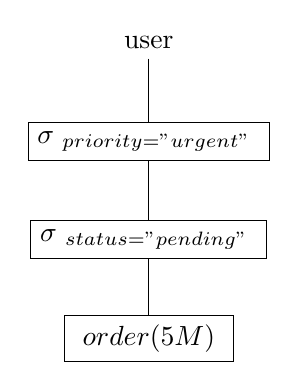
\begin{tikzpicture}[y=1.25cm]
                        \node (user) at (0, 0) {user};
                        \node[draw] (s1) at (0, -1) {$\sigma_{~priority = "urgent"~}$};
                        \node[draw] (s2) at (0, -2) {$\sigma_{~status = "pending"~}$};
                        \node[draw] (o) at (0, -3) {$~order(5M)~$};

                        \draw (user) -- (s1) -- (s2) -- (o);
                    \end{tikzpicture}
                \end{center}
                The implementation, with the previously defined selection, would be as follows;
                \begin{lstlisting}
                    Table order, buffer1, buffer2;
                    int pendingCode = 5, urgentCode = 7;
                    select(buffer1, order, pendingCode, 1);
                    select(buffer2, buffer1, urgentCode, 2);
                \end{lstlisting}
                This causes a tight loop, with no function calls nor jumps.
                This is very CPU efficient, but every operator is now a pipeline breaker, and the calculation rules are similar - each operator reads and writes all of its inputs and outputs (respectively) sequentially, and the number of pages is calculated the same as before (in the storage lecture).
                \medskip

                The calculations are quite similar to Volcano, however there's one difference in that all operators are cost-estimated completely independently, since everything is its own pipeline fragment.
                \medskip

                Consider an example with a selectivity of 25\%, 1 million tuples each with 9 32-bit attributes.
                Similarly, we have a 512 KB cache, and pages of 64 bytes.
                \begin{align*}
                    ~Selectivity~ & = 0.25 \\
                    ~CachelineSize~ & = 64 \\
                    ~BufferPoolCapacityInPages~ & = \frac{512 \cdot 1024}{64} \\
                    ~TableSizeInTuples~ & = 1000000 \\
                    ~TableTupleSize~ & = 9 \cdot 4 \\
                    ~TableSize~ & = ~TableSizeInTuples~ \cdot ~TableTupleSize~ \\
                    ~TablePages~ & = \ceil{\frac{~TableSize~}{~CachelineSize~}} \\
                    ~SelectionInputInPages~ & = ~TablePages~ \\
                    ~SelectionOutputInPages~ & = \ceil{\frac{~TableSize~ \cdot ~Selectivity~}{~CachelineSize~}} \\
                    ~SelectionIO~ & = ~SelectionInputInPages~ + ~SelectionOutputInPages~ \\
                    & = 703125
                \end{align*}
            \subsubsection*{Bulk Processing and Decomposed Storage}
                The idea of \textbf{By-Reference Bulk Processing} is to save bandwidth by avoiding copying data.
                Instead of producing tuples, we produce IDs (32-bit positions in their buffers).
                When we process a tuple, we use the ID to look up actual values - this is basically a hashtable without conflicts.
                \begin{lstlisting}
                    int select(vector<int>& outputBuffer, optional<vector<int>> const& candidatePositions, int predicate, int attributeOffset, vector<Tuple> const& underlyingRelation) {
                      // case where we are the first selection in the plan (all are candidates)
                      if (!candidatePositions.has_value()) {
                        for (size_t i = 0; i < underlyingRelation.size(); i++) {
                          if (underlyingRelation[i][attributeOffset] == predicate) {
                            outputBuffer.push_back(i);
                          }
                        }
                      } else {
                        for (size_t i = 0; i < candidatePositions->size(); i++) {
                          if (underlyingRelation[(*candidatePositions)[i]][attributeOffset] == predicate) {
                            outputBuffer[outputCursor++] = (*candidatePositions)[i];
                          }
                        }
                      }
                      return outputCursor;
                    }
                \end{lstlisting}
                The implementation of our previous result would now be as follows (note that the code above might be \textit{slightly} incorrect);
                \begin{lstlisting}
                    vector<Tuple> order;
                    vector<int> buffer1, buffer2;
                    int pendingCode = 5, urgentCode = 7;
                    auto buffer1Size = select(buffer1, {}, pendingCode, 1, order);
                    auto buffer2Size = select(buffer2, buffer1, urgentCode, 2, order);
                \end{lstlisting}
                The rules for estimating buffer I/O are slightly different; we now read all of its \textbf{candidate buffer} and write all of its candidate buffer sequentially, although the calculation remains the same.
                In addition, each operator resolves the candidate references by looking up the values in the base relation.
                The rules for temporary buffers are the same (again).
            \subsubsection*{Page Access Probability}
                If we define the selectivity $s$ as the percentage of tuples being touched, and $n$ the number of tuples on a page, and also assume uniformly distributed values, we can define the probability of any one of them being touched as;
                $$p(s, n) = 1 - (1 - s)^n$$
                We can then estimate the number of page faults as;
                $$p(~FirstSelectSelectivity~, ~AverageBaseTableTuplesPerPage~) \cdot ~BaseTablePages~$$
            \subsubsection*{By-Reference Bulk Processing of Decomposed Data}
                We can save even more bandwidth.
                We know that every operator processes exactly one column of a tuple.
                As such, N-ary storage is quite wasteful (since values of a tuple are co-located on a page), therefore we will pay the cost to access all values on a page, even if we only process one (this will also occupy space in the buffer pool).
                DSM fixes this; this was introduced as a consequence of bulk processing.
                Using the same example as before, with the selectivity of 30\%;
                \begin{align*}
                    ~SelectSelectivity~ & = 0.3 \\
                    ~CachelineSize~ & = 64 \\
                    ~BufferPoolCapacityInPages~ & = \frac{512 \cdot 1024}{64} \\
                    ~OrderTableSizeInTuples~ & = 10000 \\
                    ~OrderTupleAttributeSize~ & = 1 \cdot 4 & \text{only one attribute}
                \end{align*}
                We can then work out the sizes for the order table;
                \begin{align*}
                    ~OrderTableColumnSize~ & = ~OrderTupleAttributeSize~ \cdot ~OrderTableSizeInTuples~ \\
                    ~OrderTableColumnPages~ & = \ceil{\frac{~OrderTableColumnSize~}{~CachelineSize~}}
                \end{align*}
                Now we can look at the sizes for the selection - note that the output is actually the candidate positions, however we don't need to even consider it in our calculation (last line);
                \begin{align*}
                    ~SelectionInputInPages~ & = ~OrderTableColumnPages~ \\
                    ~SelectionOutputInTuples~ & = ~OrderTableSizeInTuples~ \cdot ~SelectSelectivity~ \\
                    ~SelectionOutputInPages~ & = \ceil{\frac{~SelectionOutputInTuples~ \cdot 4}{~CachelineSize~}} \\
                    ~SelectionIO~ & = ~SelectionInputInPages~
                \end{align*}
                For the grouping, we need to first calculate the hash table size (note that this combined with the selection output is still smaller than the buffer pool capacity, hence we can ignore it again);
                $$~GroupingHashTableSize~ = \ceil{2 \cdot ~GroupingCardinality~ \cdot ~NumberOfAttributesInGroupingTable~ \cdot 4}$$
                \begin{align*}
                    ~OrderTuplesPerPage~ & = \frac{~CachelineSize~}{~OrderTupleAttributeSize~} \\
                    ~GroupingIO~ & = \ceil{p(~SelectSelectivity~, ~OrderTuplesPerPage~) \cdot ~OrderTableColumnPages~} \\
                    & + \ceil{\frac{9 \cdot 2 \cdot 4}{~CachelineSize~}}
                \end{align*}
                Therefore our total IO is 1438.
        \subsection*{Topic 0 - Introduction}
            A distributed database is several databases at different sites, connected by server racks, LAN, or the Internet.
            This adds considerations such as network bottlenecks and failures.
            \medskip

            We can prove that there's no finite protocol where we can be certain that two sites agree on an update to a value.
            If we assume some finite chain, of $n$ messages, then the final one is not needed (since that may be unreliable), hence we have $n - 1$, and so on until we can show there are no messages in this protocol.
            \subsubsection*{CAP Theorem}
                This leads to the CAP theorem, where no distributed system can contain \textbf{all three} of the following properties;
                \begin{itemize}
                    \itemsep0em
                    \item \textbf{consistency} \hfill all nodes see the same version of data
                    \item \textbf{availability} \hfill the system always responds within a fixed upper limit of time
                    \item \textbf{partition tolerance}
                        \subitem system always gives correct responses even when messages are lost or network failures occur
                \end{itemize}
                We can have \textbf{CA} with a single system (a centralised database), \textbf{CP} with a traditional distributed RDBMS.
                The latter waits if the network becomes partitioned (until it recovers), therefore we lose availability.
                \textbf{AP} is available in some Internet protocols such as DNS, where we sacrifice consistency.
            \subsubsection*{Approaches to Distributed Databases}
                There are generally two approaches to DDB;
                \begin{itemize}
                    \itemsep0em
                    \item \textbf{Heterogeneous}
                        \smallskip

                        These vary in database technologies (and are managed by different database administrators), and are designed at different times.
                        Some example technologies are ODBC or JDBC.
                        \medskip

                        One consideration for this is that there may be different structures between the databases (for example RDBMS queried with SQL versus a CSV file queried by reading the file), and therefore a common data model (CDM) is required between them.
                        Another consideration is a semantic difference, for example a table for bank branches may have different names for the fields, and may omit the prefix of a sort code - this requires \textbf{schema integration}.
                        \medskip

                        The diagram for the heterogeneous
                    \item \textbf{Homogeneous}
                        \smallskip

                        On the other hand, this is designed at the same time, and all use the same database technology.
                        An example of this is an RDBMS cluster, or Map Reduce (e.g. Hadoop).
                        \begin{center}
                            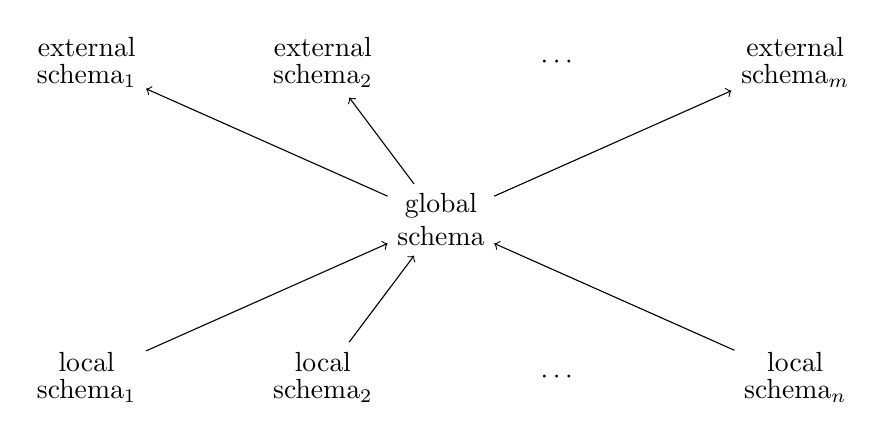
\begin{tikzpicture}[x=3cm]
                                \node (gs) at (0, 0) {\shortstack{global\\schema}};
                                \node (ls1) at (-1.5, -2) {\shortstack{local\\schema$_1$}};
                                \node (ls2) at (-0.5, -2) {\shortstack{local\\schema$_2$}};
                                \node at (0.5, -2) {$\cdots$};
                                \node (lsn) at (1.5, -2) {\shortstack{local\\schema$_n$}};
                                \node (es1) at (-1.5, 2) {\shortstack{external\\schema$_1$}};
                                \node (es2) at (-0.5, 2) {\shortstack{external\\schema$_2$}};
                                \node at (0.5, 2) {$\cdots$};
                                \node (esm) at (1.5, 2) {\shortstack{external\\schema$_m$}};

                                \draw
                                (ls1) edge[->] (gs)
                                (ls2) edge[->] (gs)
                                (lsn) edge[->] (gs)
                                (es1) edge[<-] (gs)
                                (es2) edge[<-] (gs)
                                (esm) edge[<-] (gs);
                            \end{tikzpicture}
                        \end{center}
                \end{itemize}
            \subsubsection*{Operational Model}
                In the mediator architecture, we have the following, where virtual data is represented in \teal{teal} and materialised data is represented in \violet{violet} - note that the mediators are the two that are virtual data, and the three wrappers are the materialised data.
                \medskip

                On the other hand, in the data warehouse approach, they are all materialised data (and the two that were previously teal are the data warehouses).
                Note that mediators request from the source, whereas database warehouses store the data from the source (hence materialised).
                \medskip

                Both approaches have advantages and disadvantages, but it's important to note that the global schema in a data warehouse is essentially a cache and therefore needs to be updated.
                On the other hand, using virtual data increases the traffic and load since more queries have to be made to the local schemas (and wrappers).
                \begin{center}
                    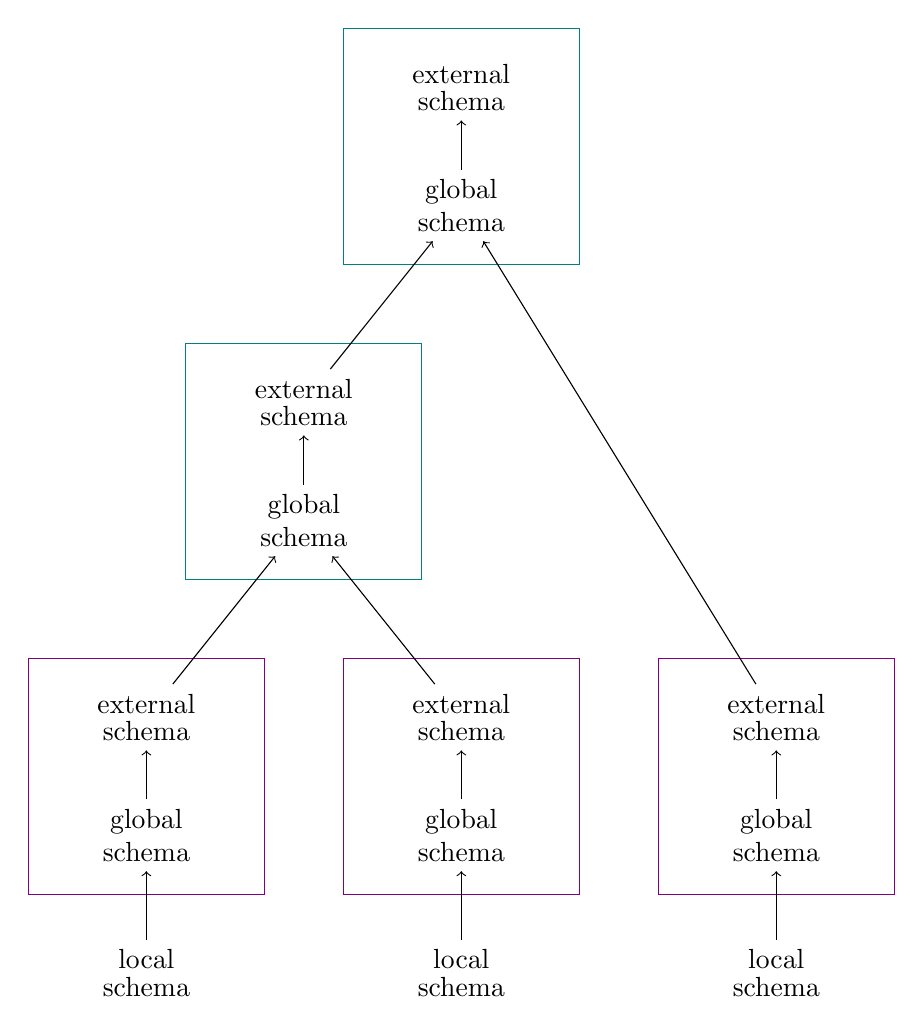
\begin{tikzpicture}
                        \begin{scope}[shift={(0, 0)}]
                            \draw[teal] (-1.5, 1.5) -- (1.5, 1.5) -- (1.5, -1.5) -- (-1.5, -1.5) -- cycle;
                            \node (es0) at (0, 0.75) {\shortstack{external\\schema}};
                            \node (gs0) at (0, -0.75) {\shortstack{global\\schema}};
                            \draw (gs0) edge[->] (es0);
                        \end{scope}
                        \begin{scope}[shift={(-2, -4)}]
                            \draw[teal] (-1.5, 1.5) -- (1.5, 1.5) -- (1.5, -1.5) -- (-1.5, -1.5) -- cycle;
                            \node (es1) at (0, 0.75) {\shortstack{external\\schema}};
                            \node (gs1) at (0, -0.75) {\shortstack{global\\schema}};
                            \draw (gs1) edge[->] (es1);
                        \end{scope}
                        \begin{scope}[shift={(-4, -8)}]
                            \draw[violet] (-1.5, 1.5) -- (1.5, 1.5) -- (1.5, -1.5) -- (-1.5, -1.5) -- cycle;
                            \node (es2) at (0, 0.75) {\shortstack{external\\schema}};
                            \node (gs2) at (0, -0.75) {\shortstack{global\\schema}};
                            \draw (gs2) edge[->] (es2);
                        \end{scope}
                        \begin{scope}[shift={(0, -8)}]
                            \draw[violet] (-1.5, 1.5) -- (1.5, 1.5) -- (1.5, -1.5) -- (-1.5, -1.5) -- cycle;
                            \node (es3) at (0, 0.75) {\shortstack{external\\schema}};
                            \node (gs3) at (0, -0.75) {\shortstack{global\\schema}};
                            \draw (gs3) edge[->] (es3);
                        \end{scope}
                        \begin{scope}[shift={(4, -8)}]
                            \draw[violet] (-1.5, 1.5) -- (1.5, 1.5) -- (1.5, -1.5) -- (-1.5, -1.5) -- cycle;
                            \node (es4) at (0, 0.75) {\shortstack{external\\schema}};
                            \node (gs4) at (0, -0.75) {\shortstack{global\\schema}};
                            \draw (gs4) edge[->] (es4);
                        \end{scope}

                        \node (ls2) at (-4, -10.5) {\shortstack{local\\schema}};
                        \node (ls3) at (0, -10.5) {\shortstack{local\\schema}};
                        \node (ls4) at (4, -10.5) {\shortstack{local\\schema}};

                        \draw
                        (ls2) edge[->] (gs2)
                        (ls3) edge[->] (gs3)
                        (ls4) edge[->] (gs4)
                        (es2) edge[->] (gs1)
                        (es3) edge[->] (gs1)
                        (es4) edge[->] (gs0)
                        (es1) edge[->] (gs0);
                    \end{tikzpicture}
                \end{center}
        \subsection*{Topic 1 - Data Distribution}
            A running example for this are the following tables;
            \begin{itemize}
                \itemsep0em
                \item ~branch~
                    \begin{itemize}
                        \itemsep0em
                        \item ~sortcode~ (key)
                        \item ~bname~ (key)
                        \item ~cash~
                    \end{itemize}
                \item ~account~
                    \begin{itemize}
                        \itemsep0em
                        \item ~no~ (key)
                        \item ~type~
                        \item ~cname~
                        \item ~rate?~
                        \item ~sortcode~ (foreign key to ~branch(sortcode)~)
                    \end{itemize}
                \item ~movement~
                    \begin{itemize}
                        \itemsep0em
                        \item ~mid~ (key)
                        \item ~no~ (foreign key to ~account(no)~)
                        \item ~amount~
                        \item ~date~
                    \end{itemize}
            \end{itemize}
            We can briefly look at the types of data distribution as follows;
            \begin{itemize}
                \itemsep0em
                \item \textbf{remote tables}
                    \smallskip

                    Consider a global schema $G$ with the tables $R, T, U, V$.
                    This is split into sites $S_1, S_2, S_3$ with tables $(R), (T, U), (V)$ respectively.
                    Therefore reads $r$ and writes $w$ must be distributed correspondingly.
                    For example, a $r[R], w[R], r[T], r[U]$ on $G$ becomes $r[R], w[R]$ on $S_1$, and $r[T], r[U]$ on $S_2$.
                \item \textbf{fragmentation}
                    \smallskip

                    Consider a similar global schema with the same sites.
                    The idea of fragmentation is to split objects $o_a, o_b, \dots$ of a relation $R$ between sites.
                    The distribution is similar to before, but on an object level.
                    \medskip

                    There are a few approaches to this;
                    \begin{itemize}
                        \itemsep0em
                        \item \textbf{horizontal fragmentation} \hfill $R_1 = \sigma_{P_1}R, \dots, R_n = \sigma_{P_n}R$
                            \smallskip

                            In this case, we split the table by rows, via a rule that \textbf{partitions} the data (prevents a row from being in multiple sites) and is roughly even.
                            For example, the original ~account~ table can be split into the following;
                            \begin{align*}
                                ~account~_~1~ & = \sigma_{~type == current~}~account~ \\
                                ~account~_~2~ & = \sigma_{~type != current~}~account~
                            \end{align*}
                            Compared to a single site version, the DDB is faster (since we can run multiple of the same query in parallel across the sites), but less reliable (since the chance of one of the sites failing during a long query is higher).
                            \medskip

                            The worst attribute to fragment on something that would change over time, in our example it would be ~rate~.
                        \item \textbf{derived horizontal fragmentation} \hfill $R_1 = R \ltimes S_1, \dots, R_n \ltimes S_n$
                            \smallskip

                            For this, we need to look at the semi-join;
                            $$R \ltimes T = R \bowtie \pi_{attr(R) \cap attr(T)}T$$
                            This gives us the same columns as $R$, but only with the rows that have a value in $T$.
                            For our running example, we might not have all accounts in the table $~account~ \ltimes ~movement~$, if it has nothing in ~movement~.
                            \medskip

                            This allows us to fragment the ~movement~ table as follows, thus storing the movements at the same site as the respective accounts;
                            $$~movement~_~i~ = ~movement~ \ltimes ~account~_~i~$$
                        \item \textbf{vertical fragmentation} \hfill $R_1 = \pi_{attrs_1}R, \dots, R_n = \pi_{attrs_n}R$
                            \smallskip

                            In this case we split by columns, simply with projections (however each attribute must be represented in at least one site, and there must be a key which we can join on, in this case ~no~);
                            \begin{align*}
                                ~account~_~1~ & = \pi_{~no, type, rate, sortcode~}~account~ \\
                                ~account~_~2~ & = \pi_{~no, cname~}~account~
                            \end{align*}
                        \item \textbf{hybrid fragmentation}
                            \smallskip

                            We can also combine the methods to fragment it further.
                    \end{itemize}
                \item \textbf{replication}
                    \smallskip

                    Consider \textbf{objects} $o_a, o_b, \dots$ on a global schema $G$.
                    We can copy the data to all the sites, such that all sites $S_1, S_2, \dots$ have a full copy of all objects.
                    This allows queries to be run on \textbf{any} site, however updates will now need to write to \textbf{all} sites.
                    \medskip

                    A query on this is faster (in the parallel case) and is more reliable (due to site redundancy) than a single site.
                    On the other hand, writes are slower but still more reliable.
                    The writes need to be coordinated, thus causing it to be slower.
                    However, the reliability of this depends on the implementation - if we do a synchronisation and one site goes down, the entire query fails.
                    On the other hand, if we are able to recover from failure (and allow the rest of the query to continue after a site has been marked down), it can be more reliable with a recovery mechanism.
                \item \textbf{migration}
            \end{itemize}
        \subsection*{Topic 2 - Big Data}
            The traditional approach to dealing with larger amounts of data was to scale up (with larger, more powerful computers).
            However, this becomes increasingly more expensive, and will often require specialist hardware.
            The more modern approach is to scale out, which is to increase the number of commodity computers to spread the data.
            \subsubsection*{Big Data System}
                A big data system is able to handle more data than fits on a single commodity computer and data that is spread over hundreds or thousands of servers.
                It must also handle the failures of nodes without any loss of data.
                As a consequence of the CAP theorem, availability is prioritised over consistency.
                \begin{center}
                    \begin{tikzpicture}
                        \draw
                        (0, 1) edge[above] node{LAN} (14, 1)
                        (1, 1) -- (1, 0)
                        (4, 1) -- (4, 0)
                        (10, 1) -- (10, 0)
                        (13, 1) -- (13, 0);
                        \begin{scope}[shift={(0, 0)}]
                            \draw (0, 0) -- (2, 0) -- (2, -3) -- (0, -3) -- cycle;
                            \draw (0.5, -0.5) -- (1.5, -0.5) -- (1.5, -2) -- (0.5, -2) -- cycle;
                            \node at (1, -1.25) {$S_1$};
                            \node at (1, -2.5) {$H_1$};
                        \end{scope}
                        \begin{scope}[shift={(3, 0)}]
                            \draw (0, 0) -- (2, 0) -- (2, -3) -- (0, -3) -- cycle;
                            \draw (0.5, -0.5) -- (1.5, -0.5) -- (1.5, -2) -- (0.5, -2) -- cycle;
                            \node at (1, -1.25) {$S_2$};
                            \node at (1, -2.5) {$H_2$};
                        \end{scope}
                        \begin{scope}[shift={(6, 0)}]
                            \node at (1, -1.5) {$\cdots$};
                        \end{scope}
                        \begin{scope}[shift={(9, 0)}]
                            \draw (0, 0) -- (2, 0) -- (2, -3) -- (0, -3) -- cycle;
                            \draw (0.5, -0.5) -- (1.5, -0.5) -- (1.5, -2) -- (0.5, -2) -- cycle;
                            \node at (1, -1.25) {$S_{n-1}$};
                            \node at (1, -2.5) {$H_{n-1}$};
                        \end{scope}
                        \begin{scope}[shift={(12, 0)}]
                            \draw (0, 0) -- (2, 0) -- (2, -3) -- (0, -3) -- cycle;
                            \draw (0.5, -0.5) -- (1.5, -0.5) -- (1.5, -2) -- (0.5, -2) -- cycle;
                            \node at (1, -1.25) {$S_n$};
                            \node at (1, -2.5) {$H_n$};
                        \end{scope}
                    \end{tikzpicture}
                \end{center}
            \subsubsection*{Data Models and MapReduce}
                Before we look at MapReduce, we should consider the different data models;
                \begin{itemize}
                    \itemsep0em
                    \item \textbf{Key-Value}
                        \smallskip

                        In this model data is stored as key-value pairs.
                        This is schema-less, and has very limited querying capabilities (but useful for implementing cache).
                        Examples of this are \textit{Memcache} or \textit{Redis}.
                    \item \textbf{Document}
                        \smallskip

                        While this has some structure to it, such as JSON, it's still schema-less as we aren't forced to a single structure.
                        This supports some queries for searching fields within a document, but cannot perform queries such as joins.
                        As such, MapReduce is used for OLAP.
                        Some examples of this are \textit{CouchDB} or \textit{MongoDB}.
                    \item \textbf{Wide Column}
                        \smallskip

                        Table data model with easy addition of new columns, and columns are put into families (allowing for vertical fragmentation on families).
                        Also schema-less, and supports queries searching field values.
                        MapReduce is also used for OLAP.
                    \item \textbf{Relational}
                        \smallskip

                        Schema based, and supports queries for searching fields and joins.
                        Has ACID properties.
                    \item \textbf{Graph} \hfill schema-less
                \end{itemize}
                The general structure of MapReduce is as follows;
                \begin{center}
                    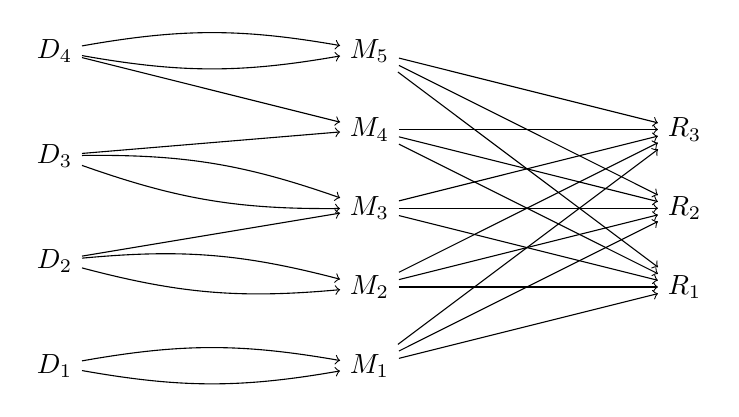
\begin{tikzpicture}[x=2cm]
                        \node (d4) at (0, 0) {$D_4$};
                        \node (d3) at (0, -1.333) {$D_3$};
                        \node (d2) at (0, -2.666) {$D_2$};
                        \node (d1) at (0, -4) {$D_1$};
                        \node (m5) at (2, 0) {$M_5$};
                        \node (m4) at (2, -1) {$M_4$};
                        \node (m3) at (2, -2) {$M_3$};
                        \node (m2) at (2, -3) {$M_2$};
                        \node (m1) at (2, -4) {$M_1$};
                        \node (r3) at (4, -1) {$R_3$};
                        \node (r2) at (4, -2) {$R_2$};
                        \node (r1) at (4, -3) {$R_1$};

                        \draw
                        (d4) edge[->, bend left=10] (m5)
                        (d4) edge[->, bend right=10] (m5)
                        (d4) edge[->] (m4)
                        (d3) edge[->, bend left=10] (m3)
                        (d3) edge[->, bend right=10] (m3)
                        (d3) edge[->] (m4)
                        (d2) edge[->, bend left=10] (m2)
                        (d2) edge[->, bend right=10] (m2)
                        (d2) edge[->] (m3)
                        (d1) edge[->, bend left=10] (m1)
                        (d1) edge[->, bend right=10] (m1)
                        (m5) edge[->] (r3)
                        (m5) edge[->] (r2)
                        (m5) edge[->] (r1)
                        (m4) edge[->] (r3)
                        (m4) edge[->] (r2)
                        (m4) edge[->] (r1)
                        (m3) edge[->] (r3)
                        (m3) edge[->] (r2)
                        (m3) edge[->] (r1)
                        (m2) edge[->] (r3)
                        (m2) edge[->] (r2)
                        (m2) edge[->] (r1)
                        (m1) edge[->] (r3)
                        (m1) edge[->] (r2)
                        (m1) edge[->] (r1);
                    \end{tikzpicture}
                \end{center}
                Between the data nodes and the map nodes is the load phase, and between the map nodes and the reduce nodes is the shuffle phase.
                A hash function is used by the map nodes to decide which reduce nodes to to pass the data into in the shuffle phase (or some sort of rule that is known by all the map nodes).
                \medskip

                We might notice that some of the work can be done in the map nodes (for example counting words), and this introduces the \textbf{combine} operation, which is a partial reduction, this reduces the inefficiency between the map nodes and the reduce nodes.
                \medskip

                In the word count example, we have the following actions;
                \begin{itemize}
                    \itemsep0em
                    \item map \hfill obtain all words as a pair with a 1 (count)
                    \item combine \hfill partially reduce to give a word with a frequency
                    \item reduce \hfill fully reduce with all map nodes
                \end{itemize}
                MapReduce was originally reported by Google, and an open source implementation with the Hadoop family is as follows;
                \begin{itemize}
                    \itemsep0em
                    \item Hadoop Distributed File System (HDFS)
                        \smallskip

                        Standard storage by Hadoop applications, fragmentation by default in 128MB blocks, and defaults to three nodes of replication.
                    \item Hadoop \hfill  Java implementation of MapReduce
                    \item Hive \hfill SQL language translated into Hadoop applications
                    \item Pig Latin \hfill high level scripting language to write Hadoop applications
                    \item HBase \hfill Java API to provide big table, provides scalable read / write access
                \end{itemize}
        \subsection*{Topic 3 - Pig Latin (RA)}
            \subsubsection*{Accessing Data}
                The ~LOAD~ operator reads in a TSV (by default) file as a relation.
                \begin{lstlisting}
                    account =
                        LOAD '/path/to/account.tsv'
                        AS (no:int, type:chararray, cname:chararray, rate:float, sortcode:int);
                \end{lstlisting}
            \subsubsection*{Relational Algebra}
                Some of the basic components of the relational algebra are implemented in Pig Latin as follows;
                \begin{itemize}
                    \itemsep0em
                    \item project ($\pi$) \hfill $\pi_{~sortcode~}$ - ~FOREACH <ALIAS> GENERATE <COLNAME>, ...~
                        \begin{lstlisting}
                            account_sortcode_bag =
                                FOREACH account
                                GENERATE sortcode;

                            account_sortcode =
                                DISTINCT account_sortcode_bag; # set
                        \end{lstlisting}
                    \item select ($\sigma$) \hfill $\sigma_{~rate>0~}$ - ~FILTER <ALIAS> BY <PREDICATE>~
                        \begin{lstlisting}
                            account_with_rate =
                                FILTER account
                                BY rate > 0.0;
                        \end{lstlisting}
                    \item product ($\times$) \hfill ~CROSS <ALIAS> <ALIAS>~
                        \begin{lstlisting}
                            branch_account_with_rate =
                                CROSS branch, account_with_rate;
                        \end{lstlisting}
                    \item join ($\bowtie$) - only performs equi-joins \hfill ~JOIN <ALIAS> BY <COLNAME>, <ALIAS> BY <COLNAME>~
                        \begin{lstlisting}
                            branch_with_interest_account =
                                JOIN branch by branch::sortcode,
                                     account_with_rate BY account_with_rate::sortcode;
                        \end{lstlisting}
                    \item union ($\cup$) \hfill $\pi_~sortcode~~branch~ \cup \pi_~no~~account~$ - ~UNION <ALIAS>, <ALIAS>~
                        \begin{lstlisting}
                            branch_sortcode =
                                FOREACH branch
                                GENERATE sortcode;
                            account_no =
                                FOREACH account
                                GENERATE no;
                            all_ids_bag =
                                UNION branch_sortcode, account_no;
                            all_ids =
                                DISTINCT all_ids_bag;
                        \end{lstlisting}
                    \item difference ($-$)
                        \subitem

                        Note that here there is no direct implementation.
                        It has be to done by performing a left join and then keeping rows with null values.
                        For example, performing the following;
                        $$\pi_~no~~account~ - \pi_~no~~movement~$$
                        \begin{lstlisting}
                            account_and_movement =
                                JOIN account BY no LEFT,
                                movement BY no;
                            account_without_movement =
                                FILTER account_and_movement
                                BY movement::no IS NULL;
                            account_no_without_movement =
                                FOREACH account_without_movement
                                GENERATE no;
                        \end{lstlisting}
                \end{itemize}
        \subsection*{Topic 4 - Pig Latin (Aggregation)}
            For this, we need to look at ~GROUP~ and ~FLATTEN~ (which reverts a ~GROUP~).
            Note that when a group is made, it creates two columns ~group~ (which contains the attribute key we're grouping on), and ~<ALIAS>~, which contains a bag of tuples (from the original relation).
            \begin{lstlisting}
                accounts_movement =
                    GROUP movement
                    BY no;

                movement_copy =
                    FOREACH account_movements
                    GENERATE FLATTEN(movement)

                account_balance =
                    FOREACH account_movements
                    GENERATE group AS no, # rename
                             SUM(movement.amount) AS balance; # accesses bag structure
            \end{lstlisting}
            The aggregation operators available to us are as follows;
            \begin{center}
                \begin{tabular}{l|l}
                    function & result \\
                    \hline
                    ~int COUNT(bag)~ & returns the number of \textbf{not null} values in the bag \\
                    ~int COUNT\_STAR(bag)~ & returns the number of values in the bag (\textbf{including null}) \\
                    ~double AVG(bag)~ & returns the average of the values in the bag \\
                    ~double MAX(bag)~ & returns the maximum value in the bag \\
                    ~double MIN(bag)~ & returns the minimum value in the bag \\
                    ~double SUM(bag)~ & returns the sum of the values in the bag \\
                    ~bag DIFF(bag a, bag b)~ & returns tuples in ~a~ that do not appear in ~b~
                \end{tabular}
            \end{center}
            To achieve something similar to SQL, we need to use the ~GROUP~ operator, and then apply the aggregation operators to the bag of tuples.
            \medskip

            To optimise the previous query, we can reduce the amount of elements we store (if we aren't using them);
            \begin{lstlisting}
                movement_data =
                    FOREACH movement,
                    GENERATE no, amount;

                accounts_movement =
                    GROUP movement_data
                    BY no;

                account_balance =
                    FOREACH account_movements
                    GENERATE group AS no,
                             SUM(movement.amount) AS balance;
            \end{lstlisting}
            The above will give the same result, but the ~accounts\_movement~ relation will be much smaller, we will only preserve the ~amount~ field.
            \subsubsection*{Nested Statements}
                The following is a statement in SQL;
                \begin{lstlisting}
                    SELECT   account.no
                             COUNT(movement.mid) AS no_trans,
                             SUM(CASE WHEN amount > 0.0 THEN amount ELSE 0.0 END) AS credit,
                             SUM(CASE WHEN amount < 0.0 THEN amount ELSE 0.0 END) AS debit,
                    FROM     account LEFT JOIN movement ON account.no=movement.no
                    GROUP BY account.no
                \end{lstlisting}
                Converted to Pig Script, we have the following;
                \begin{lstlisting}
                    account_and_movement =
                        JOIN account BY no LEFT,
                             movement BY no;
                    account_detail =
                        GROUP account_and_movement BY account::no;
                    account_credits_and_debits =
                        FOREACH account_detail {
                            credit =
                                FILTER account_and_movement
                                BY     amount > 0.0;
                            debit =
                                FILTER account_and_movement
                                BY     amount < 0.0;
                            GENERATE group AS no,
                                     COUNT(account_and_movement) AS no_trans,
                                     SUM(credit.amount) AS credit,
                                     SUM(debit.amount) AS debit;
                        }
                \end{lstlisting}
            \subsubsection*{WHERE and HAVING}
                Consider the following example in SQL;
                \begin{lstlisting}
                    SELECT account.cname,
                           SUM(movement.amount) AS balance
                    FROM account
                         JOIN movement ON account.no=movement.no
                    WHERE ABS(movement.amount)>100
                    GROUP BY account.cname
                    HAVING SUM(movement.amount)>200
                \end{lstlisting}
                In Pig, the same query would be done as follows;
                \begin{lstlisting}
                    account_movement_join =
                        JOIN account BY no, movement BY no;

                    account_movement_large =
                        FILTER account_movement_join
                        BY ABS(amount) > 100;

                    # optimisation
                    account_movement =
                        FOREACH account_movement_large
                        GENERATE cname, amount;

                    customer_details =
                        GROUP account_movement BY account::cname;

                    customer_balance_all =
                        FOREACH customer_details
                        GENERATE group AS cname, SUM(account_movement.movement::amount) AS balance;

                    customer_balance_large =
                        FILTER customer_balance_all
                        BY balance > 200
                \end{lstlisting}
        \subsection*{Lecture 5 - Pig Latin (MapReduce)}
            Pig scripts are interpreted into a sequence of Hadoop Map, Combine, Shuffle, and Reduce operations.
            Typically, Map and Combine processes are run on the nodes which contain data.
            The number of Reduce nodes is specified in Pig script, and defaults to 1.
            Temporary files are used to allow output of one MapReduce process to be fed into another.
            The only optimisation that is done by the Pig interpreter is to automatically push projections (from ~GENERATE~ in Pig) inside joins, anything else should be done by the script author.
            The translations are as follows;
            \begin{center}
                \begin{tabular}{ll}
                    Pig operator & map / reduce \\
                    \hline
                    $~FILTER ~ R ~ BY ~ A == val$ & map \\
                    $~FOREACH ~ R ~ GENERATE ~ A, B, \dots$ & map \\
                    $~CROSS ~ R, S$ & reduce \\
                    $~GROUP ~ R ~ BY ~ A$ & combine (if possible), reduce \\
                    $~JOIN ~ R ~ BY ~ A, S ~ BY ~ B$ & reduce \\
                    $~JOIN ~ R ~ BY ~ A ~ LEFT OUTER~, S ~ BY ~ B$ & reduce \\
                    $~JOIN ~ R ~ BY ~ A ~ RIGHT OUTER~, S ~ BY ~ B$ & reduce \\
                    $~UNION ~ R, S$ & reduce
                \end{tabular}
            \end{center}
            The number of reduce nodes can be controlled by a ~PARALLEL~ option at the end of the reduce operator.
            \subsubsection*{Distributed Hash Join}
                The standard ~JOIN~ will hash the value and send it to the correct hash bucket, note that for three reduce nodes, there are three corresponding buckets.
                The following diagram represents ~JOIN r BY a, s BY b~ with three reduce nodes.
                \begin{center}
                    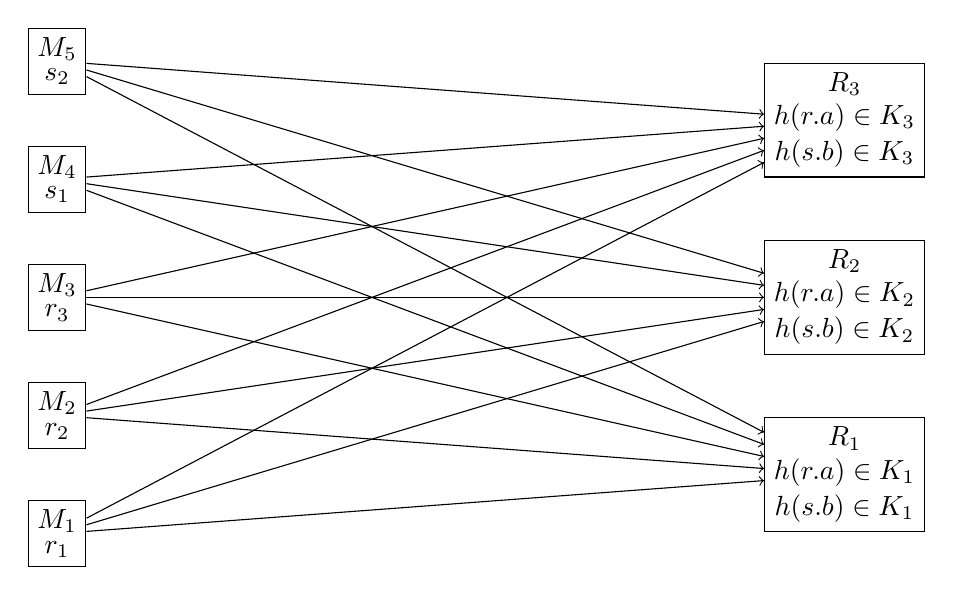
\begin{tikzpicture}[y=1.5cm]
                        \node[draw] (m5) at (0, 0) {\shortstack{$M_5$\\$s_2$}};
                        \node[draw] (m4) at (0, -1) {\shortstack{$M_4$\\$s_1$}};
                        \node[draw] (m3) at (0, -2) {\shortstack{$M_3$\\$r_3$}};
                        \node[draw] (m2) at (0, -3) {\shortstack{$M_2$\\$r_2$}};
                        \node[draw] (m1) at (0, -4) {\shortstack{$M_1$\\$r_1$}};

                        \node[draw] (r3) at (10, -0.5) {\shortstack{$R_3$\\$h(r.a) \in K_3$\\$h(s.b) \in K_3$}};
                        \node[draw] (r2) at (10, -2) {\shortstack{$R_2$\\$h(r.a) \in K_2$\\$h(s.b) \in K_2$}};
                        \node[draw] (r1) at (10, -3.5) {\shortstack{$R_1$\\$h(r.a) \in K_1$\\$h(s.b) \in K_1$}};

                        \draw
                        (m5) edge[->] (r3)
                        (m5) edge[->] (r2)
                        (m5) edge[->] (r1)
                        (m4) edge[->] (r3)
                        (m4) edge[->] (r2)
                        (m4) edge[->] (r1)
                        (m3) edge[->] (r3)
                        (m3) edge[->] (r2)
                        (m3) edge[->] (r1)
                        (m2) edge[->] (r3)
                        (m2) edge[->] (r2)
                        (m2) edge[->] (r1)
                        (m1) edge[->] (r3)
                        (m1) edge[->] (r2)
                        (m1) edge[->] (r1);
                    \end{tikzpicture}
                \end{center}
            \subsubsection*{Replicated Join}
                In a replicated join, the entire right hand table can be copied to all the map nodes holding the left hand table.
                These replicated joins are then executed as a Map process.
                The following diagram represents ~JOIN r BY a, s BY b USING 'replicated'~, where ~s~ only resides on one map node;
                \begin{center}
                    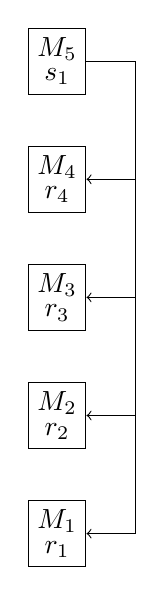
\begin{tikzpicture}[y=1.5cm]
                        \node[draw] (m5) at (0, 0) {\shortstack{$M_5$\\$s_1$}};
                        \node[draw] (m4) at (0, -1) {\shortstack{$M_4$\\$r_4$}};
                        \node[draw] (m3) at (0, -2) {\shortstack{$M_3$\\$r_3$}};
                        \node[draw] (m2) at (0, -3) {\shortstack{$M_2$\\$r_2$}};
                        \node[draw] (m1) at (0, -4) {\shortstack{$M_1$\\$r_1$}};

                        \draw
                        (1, 0) -- (1, -4)
                        (1, 0) -- (m5)
                        (1, -1) edge[->] (m4)
                        (1, -2) edge[->] (m3)
                        (1, -3) edge[->] (m2)
                        (1, -4) edge[->] (m1);
                    \end{tikzpicture}
                \end{center}
                Note that a ~RIGHT~ join cannot be done, since we cannot determine whether it joins or not on a particular node.
                For example, if we had a row in table $s$ that doesn't join on anything; each of the map nodes can be certain it doesn't join, however it doesn't know if it joins on another node.
            \subsubsection*{Skewed Join}
                In a skewed join, a histogram of the various join keys in $r$ is first generated.
                If a key has a high frequency in $r$, the rows of $r$ are distributed in a round robin fashion, and the rows of $s$ are duplicated.
                The following diagram represents ~JOIN r BY a, s BY b USING 'skewed'~;
                \begin{center}
                    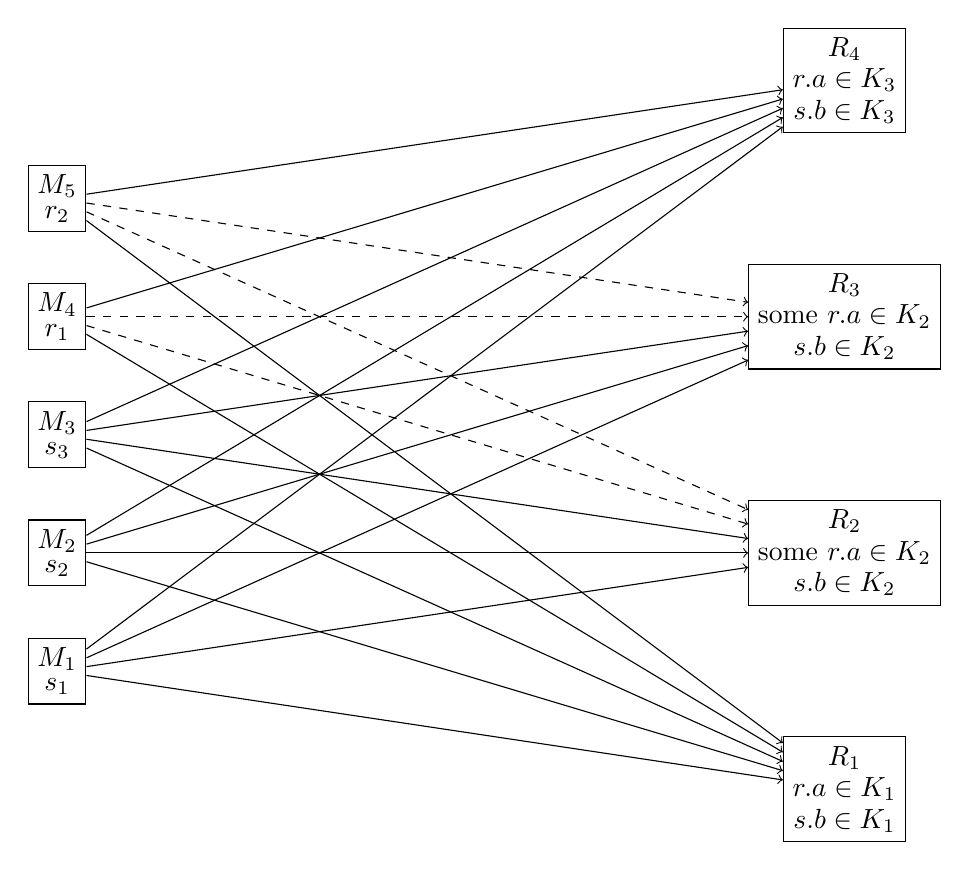
\begin{tikzpicture}[y=1.5cm]
                        \node[draw] (m5) at (0, 0) {\shortstack{$M_5$\\$r_2$}};
                        \node[draw] (m4) at (0, -1) {\shortstack{$M_4$\\$r_1$}};
                        \node[draw] (m3) at (0, -2) {\shortstack{$M_3$\\$s_3$}};
                        \node[draw] (m2) at (0, -3) {\shortstack{$M_2$\\$s_2$}};
                        \node[draw] (m1) at (0, -4) {\shortstack{$M_1$\\$s_1$}};

                        \node[draw] (r4) at (10, 1) {\shortstack{$R_4$\\$r.a \in K_3$\\$s.b \in K_3$}};
                        \node[draw] (r3) at (10, -1) {\shortstack{$R_3$\\$\text{some } r.a \in K_2$\\$s.b \in K_2$}};
                        \node[draw] (r2) at (10, -3) {\shortstack{$R_2$\\$\text{some } r.a \in K_2$\\$s.b \in K_2$}};
                        \node[draw] (r1) at (10, -5) {\shortstack{$R_1$\\$r.a \in K_1$\\$s.b \in K_1$}};

                        \draw
                        (m5) edge[->] (r4)
                        (m5) edge[->, dashed] (r3)
                        (m5) edge[->, dashed] (r2)
                        (m5) edge[->] (r1)
                        (m4) edge[->] (r4)
                        (m4) edge[->, dashed] (r3)
                        (m4) edge[->, dashed] (r2)
                        (m4) edge[->] (r1)
                        (m3) edge[->] (r4)
                        (m3) edge[->] (r3)
                        (m3) edge[->] (r2)
                        (m3) edge[->] (r1)
                        (m2) edge[->] (r4)
                        (m2) edge[->] (r3)
                        (m2) edge[->] (r2)
                        (m2) edge[->] (r1)
                        (m1) edge[->] (r4)
                        (m1) edge[->] (r3)
                        (m1) edge[->] (r2)
                        (m1) edge[->] (r1);
                    \end{tikzpicture}
                \end{center}
            \subsubsection*{Merge Join}
                This is a variation of SMJ, where it's assumed both inputs are already sorted.
                The first record of each block of $s$ are sampled to determine the layout.
                The map nodes of $r$ load $s$ blocks as required.
                The following diagram represents ~JOIN r BY a, s BY b USING 'merge'~;
                \begin{center}
                    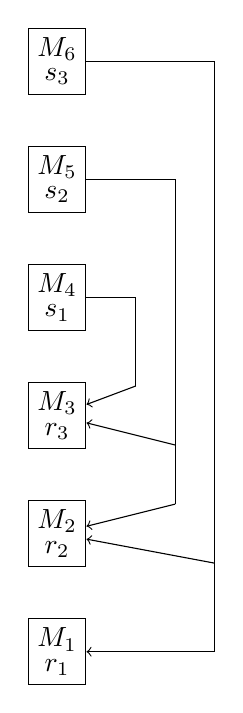
\begin{tikzpicture}[y=1.5cm]
                        \node[draw] (m6) at (0, 0) {\shortstack{$M_6$\\$s_3$}};
                        \node[draw] (m5) at (0, -1) {\shortstack{$M_5$\\$s_2$}};
                        \node[draw] (m4) at (0, -2) {\shortstack{$M_4$\\$s_1$}};
                        \node[draw] (m3) at (0, -3) {\shortstack{$M_3$\\$r_3$}};
                        \node[draw] (m2) at (0, -4) {\shortstack{$M_2$\\$r_2$}};
                        \node[draw] (m1) at (0, -5) {\shortstack{$M_1$\\$r_1$}};

                        \draw
                        (1, -2) -- (1, -2.75)
                        (1, -2) -- (m4)
                        (1, -2.75) edge[->] (m3)
                        (1.5, -1) -- (1.5, -3.75)
                        (1.5, -1) -- (m5)
                        (1.5, -3.25) edge[->] (m3)
                        (1.5, -3.75) edge[->] (m2)
                        (2, 0) -- (2, -5)
                        (2, 0) -- (m6)
                        (2, -4.25) edge[->] (m2)
                        (2, -5) edge[->] (m1);
                    \end{tikzpicture}
                \end{center}
        \subsection*{Topic 6 - Distributing Queries}
            A traditional DBMS consists of the following three components;
            \begin{itemize}
                \itemsep0em
                \item transaction manager
                    \smallskip

                    Translates queries from a higher level language to a set of primitive operations, possibly optimising them in the process.
                \item scheduler
                    \smallskip

                    Decides how to execute the aforementioned sequence of tasks concurrently to ensure the highest throughput.
                \item data manager
                    \smallskip

                    Ensures that data is sent and read from disk in the most efficient way, and maintains durability of transactions.
            \end{itemize}
            In a distributed system, each site runs a local transaction manager (LTM), scheduler and data manager.
            There can be one or more sites with a global transaction manager, which dispatches the queries (and returns any data if required) based on predefined rules.
            The slowest part of distributed query processing is the communication between sites, and we'd like to minimise the amount of data sent between sites.
            \subsubsection*{Global Transaction Manager Execution Plan}
                The GTM must transform transactions into sub-transactions for each site.
                If the table is fragmented, the transaction should be broken up into fragments (for example moving money between accounts, where the accounts reside on different databases can be done in two queries, one decrementing in the first table, another incrementing in the second).
                In the case of replicated tables, a read transaction only needs to go to one site, however any writing transactions will need to go to all sites.
                \medskip

                In this example, assuming a horizontally fragmented relation;
                \begin{lstlisting}
                    -- from GTM
                    BEGIN TRANSACTION T4
                      SELECT SUM(cash)
                      FROM branch
                    COMMIT TRANSACTION T4

                    -- sent to LTM1 (sortcode<50)
                    BEGIN TRANSACTION T4_1
                      SELECT @X=SUM(cash)
                      FROM branch
                    COMMIT TRANSACTION T4_1

                    -- sent to LTM2 (sortcode>=50)
                    BEGIN TRANSACTION T4_2
                      SELECT @Y=SUM(cash)
                      FROM branch
                    COMMIT TRANSACTION T4_2

                    -- combined at GTM
                    BEGIN TRANSACTION T4
                      SELECT @X + @Y
                    COMMIT TRANSACTION T4
                \end{lstlisting}
            \subsubsection*{RA Equivalences}
                We can use some equivalences in RA to improve our performance.
                Assume at $S_1$ we have $R_1(A, B, C)$ and $T_1(A, D, E)$, and at $S_2$ we have $R_2(A, B, C)$ and $T_2(A, D, E)$.
                At $S_3$, we want $\sigma_{A = n}R$.
                We can consider $R = R_1 \cup R_2$, hence the two are equivalent;
                \begin{center}
                    \hfill
                    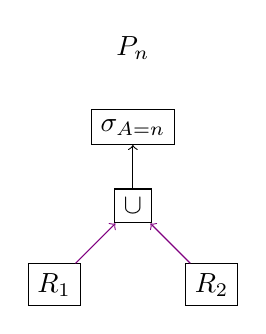
\begin{tikzpicture}
                        \node at (0, 0) {$P_n$};
                        \node[draw] (ns) at (0, -1) {$\sigma_{A = n}$};
                        \node[draw] (nu) at (0, -2) {$\cup$};
                        \node[draw] (n1) at (-1, -3) {$R_1$};
                        \node[draw] (n2) at (1, -3) {$R_2$};

                        \draw
                        (n1) edge[violet, ->] (nu)
                        (n2) edge[violet, ->] (nu)
                        (nu) edge[->] (ns);
                    \end{tikzpicture}
                    \hfill
                    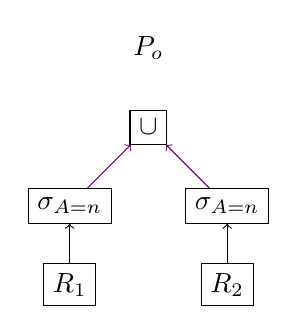
\begin{tikzpicture}
                        \node at (0, 0) {$P_o$};
                        \node[draw] (nu) at (0, -1) {$\cup$};
                        \node[draw] (ns1) at (-1, -2) {$\sigma_{A = n}$};
                        \node[draw] (ns2) at (1, -2) {$\sigma_{A = n}$};
                        \node[draw] (n1) at (-1, -3) {$R_1$};
                        \node[draw] (n2) at (1, -3) {$R_2$};

                        \draw
                        (n1) edge[->] (ns1)
                        (n2) edge[->] (ns2)
                        (ns1) edge[violet, ->] (nu)
                        (ns2) edge[violet, ->] (nu);
                    \end{tikzpicture}
                    \hfill \phantom{}
                \end{center}
                The cost of these can be analysed as follows (note that the lines in \violet{violet} represent network transfers, and NDB stands for network data bytes);
                \begin{align*}
                    NDB(P_n) & = |R| \cdot \text{RowSize}(R) \\
                    NDB(P_o) & = |\sigma_{A = n}R| \cdot \text{RowSize}(R)
                \end{align*}
                If the attribute we are selecting over, in this case $n$, is part of the partition rule (such that we have $n \in K_1$, and $R_1 = \sigma_{A \in K_1}R$ and $R_2 = \sigma_{A \in K_2}R$), we can optimise even further by only considering $R_1$.
                \medskip

                Similar logic can be applied in the case of vertical fragmentation; we can optimise a query if the columns we are considering are all in the same fragment (and therefore can ignore any other fragments).
        \subsection*{Topic 7 - Distributed Joins}
            \subsubsection*{RA Equivalences Continued}
                Assume at $S_1$ we have $R(A, B, C)$, and at $S_2$ we have $T(A, D, E)$.
                We want to obtain $\pi_{A, B, D}(R \bowtie T)$ on $S_1$ (hence we only need stuff from $S_2$ to be sent over);
                \begin{center}
                    \hfill
                    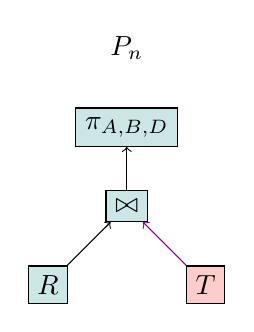
\begin{tikzpicture}
                        \node at (0, 0) {$P_n$};
                        \node[draw, fill=teal!20] (np) at (0, -1) {$\pi_{A, B, D}$};
                        \node[draw, fill=teal!20] (nj) at (0, -2) {$\bowtie$};
                        \node[draw, fill=teal!20] (n1) at (-1, -3) {$R$};
                        \node[draw, fill=red!20] (n2) at (1, -3) {$T$};

                        \draw
                        (n1) edge[->] (nj)
                        (n2) edge[violet, ->] (nj)
                        (nj) edge[->] (np);
                    \end{tikzpicture}
                    \hfill
                    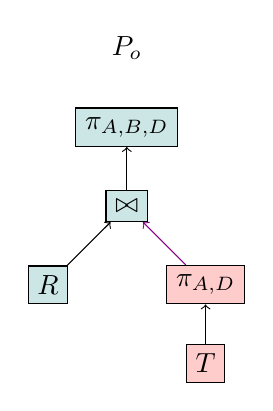
\begin{tikzpicture}
                        \node at (0, 0) {$P_o$};
                        \node[draw, fill=teal!20] (np) at (0, -1) {$\pi_{A, B, D}$};
                        \node[draw, fill=teal!20] (nj) at (0, -2) {$\bowtie$};
                        \node[draw, fill=teal!20] (n1) at (-1, -3) {$R$};
                        \node[draw, fill=red!20] (n2p) at (1, -3) {$\pi_{A, D}$};
                        \node[draw, fill=red!20] (n2) at (1, -4) {$T$};

                        \draw
                        (n1) edge[->] (nj)
                        (n2) edge[->] (n2p)
                        (n2p) edge[violet, ->] (nj)
                        (nj) edge[->] (np);
                    \end{tikzpicture}
                    \hfill \phantom{}
                \end{center}
                The cost of these can be analysed as follows;
                \begin{align*}
                    NDB(P_n) & = |T| \cdot \text{RowSize}(T) \\
                    NDB(P_o) & = |\pi_{A, D}T| \cdot \text{RowSize}(\pi_{A, D}T)
                \end{align*}
                Using the same structure, assume we now want to perform $S_1 : \sigma_{D = n}(R \bowtie T)$;
                \begin{center}
                    \hfill
                    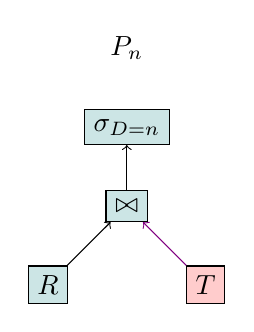
\begin{tikzpicture}
                        \node at (0, 0) {$P_n$};
                        \node[draw, fill=teal!20] (ns) at (0, -1) {$\sigma_{D = n}$};
                        \node[draw, fill=teal!20] (nj) at (0, -2) {$\bowtie$};
                        \node[draw, fill=teal!20] (n1) at (-1, -3) {$R$};
                        \node[draw, fill=red!20] (n2) at (1, -3) {$T$};

                        \draw
                        (n1) edge[->] (nj)
                        (n2) edge[violet, ->] (nj)
                        (nj) edge[->] (ns);
                    \end{tikzpicture}
                    \hfill
                    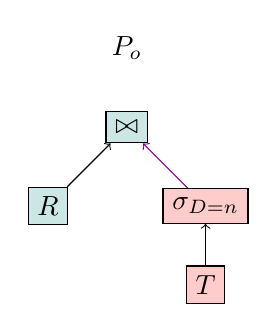
\begin{tikzpicture}
                        \node at (0, 0) {$P_o$};
                        \node[draw, fill=teal!20] (nj) at (0, -1) {$\bowtie$};
                        \node[draw, fill=teal!20] (n1) at (-1, -2) {$R$};
                        \node[draw, fill=red!20] (n2s) at (1, -2) {$\sigma_{D = n}$};
                        \node[draw, fill=red!20] (n2) at (1, -3) {$T$};

                        \draw
                        (n1) edge[->] (nj)
                        (n2) edge[->] (n2s)
                        (n2s) edge[violet, ->] (nj);
                    \end{tikzpicture}
                    \hfill \phantom{}
                \end{center}
                Similarly, we can notice that the optimised query sends less traffic (since we are reducing the number of rows we send);
                \begin{align*}
                    NDB(P_n) & = |T| \cdot \text{RowSize}(T) \\
                    NDB(P_o) & = |\sigma_{D = n}T| \cdot \text{RowSize}(T)
                \end{align*}
                Another equivalence we can consider are direct and semi joins.
                For this scenario, we want to get $R \bowtie T$ at $S_1$.
                To do so, we can ensure that we only send over the rows of $T$ that join with $R$, by first sending over the projection of $T$ that has the joining attributes.
                \begin{center}
                    \hfill
                    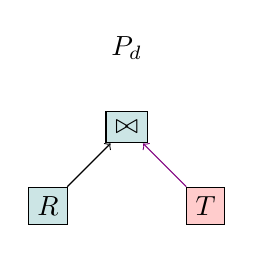
\begin{tikzpicture}
                        \node at (0, 0) {$P_d$};
                        \node[draw, fill=teal!20] (nj) at (0, -1) {$\bowtie$};
                        \node[draw, fill=teal!20] (n1) at (-1, -2) {$R$};
                        \node[draw, fill=red!20] (n2) at (1, -2) {$T$};

                        \draw
                        (n1) edge[->] (nj)
                        (n2) edge[violet, ->] (nj);
                    \end{tikzpicture}
                    \hfill
                    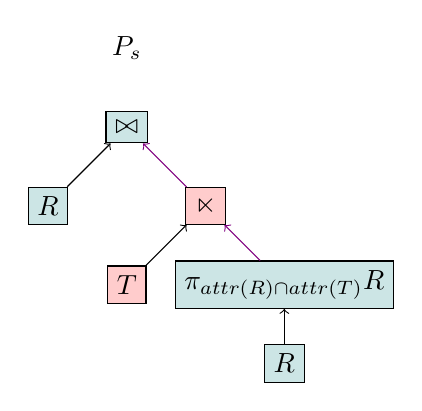
\begin{tikzpicture}
                        \node at (0, 0) {$P_s$};
                        \node[draw, fill=teal!20] (nj) at (0, -1) {$\bowtie$};
                        \node[draw, fill=teal!20] (n1) at (-1, -2) {$R$};
                        \node[draw, fill=red!20] (pj) at (1, -2) {$\ltimes$};
                        \node[draw, fill=red!20] (n2) at (0, -3) {$T$};
                        \node[draw, fill=teal!20] (p) at (2, -3) {$\pi_{attr(R) \cap attr(T)}R$};
                        \node[draw, fill=teal!20] (n12) at (2, -4) {$R$};

                        \draw
                        (n1) edge[->] (nj)
                        (pj) edge[violet, ->] (nj)
                        (n2) edge[->] (pj)
                        (p) edge[violet, ->] (pj)
                        (n12) edge[->] (p);
                    \end{tikzpicture}
                    \hfill \phantom{}
                \end{center}
                This gives us a resultant NDB as follows;
                \begin{align*}
                    NDB(P_d) & = |T| \cdot \text{RowSize}(T) \\
                    NDB(P_s) & = |\pi_{attr(R) \cap attr(T)}R| \cdot \text{RowSize}(\pi_{attr(R) \cap attr(T)}R) + |T \ltimes R| \cdot \text{RowSize}(T)
                \end{align*}
                It's important to note that this isn't always optimal, and therefore shouldn't always be applied (doing the first transfer can be wasteful).
                \medskip

                For this example, where we consider \textbf{local and remote} joins, we have another relation in $S_2$, which is $U(E, F, G)$.
                Our goal is to obtain $S_1 : R \bowtie T \bowtie U$;
                \begin{center}
                    \hfill
                    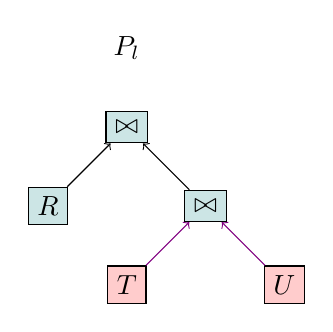
\begin{tikzpicture}
                        \node at (0, 0) {$P_l$};
                        \node[draw, fill=teal!20] (nj0) at (0, -1) {$\bowtie$};
                        \node[draw, fill=teal!20] (n1) at (-1, -2) {$R$};
                        \node[draw, fill=teal!20] (nj1) at (1, -2) {$\bowtie$};
                        \node[draw, fill=red!20] (n2) at (0, -3) {$T$};
                        \node[draw, fill=red!20] (n3) at (2, -3) {$U$};

                        \draw
                        (n1) edge[->] (nj0)
                        (nj1) edge[->] (nj0)
                        (n2) edge[violet, ->] (nj1)
                        (n3) edge[violet, ->] (nj1);
                    \end{tikzpicture}
                    \hfill
                    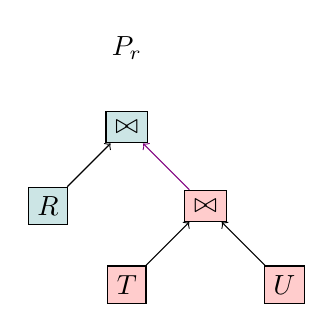
\begin{tikzpicture}
                        \node at (0, 0) {$P_r$};
                        \node[draw, fill=teal!20] (nj0) at (0, -1) {$\bowtie$};
                        \node[draw, fill=teal!20] (n1) at (-1, -2) {$R$};
                        \node[draw, fill=red!20] (nj1) at (1, -2) {$\bowtie$};
                        \node[draw, fill=red!20] (n2) at (0, -3) {$T$};
                        \node[draw, fill=red!20] (n3) at (2, -3) {$U$};

                        \draw
                        (n1) edge[->] (nj0)
                        (nj1) edge[violet, ->] (nj0)
                        (n2) edge[->] (nj1)
                        (n3) edge[->] (nj1);
                    \end{tikzpicture}
                    \hfill \phantom{}
                \end{center}
                If we move the one of the joins onto the local server, we have the following;
                \begin{align*}
                    NDB(P_l) & = |T| \cdot \text{RowSize}(T) + |U| \cdot \text{RowSize}(U) \\
                    NDB(P_r) & = |T \bowtie U| \cdot \text{RowSize}(T \bowtie U)
                \end{align*}
                Similar to before, we cannot always be certain that this will offer an improvement.
                \medskip

                Another equivalence to consider is a join over a derived horizontal fragmentation.
                Assume we wanted to obtain $\blue{S_3 : R \bowtie T}$ and $T_n = T \ltimes R_n$, with $R_n(A, B, C)$ and $T_n(A, D, E)$ at \teal{$S_1$} and \red{$S_2$}.
                Instead of performing the join after taking the union ($R_1 \cup R_2$ and $T_1 \cup T_2$), the join could be done on each of the remotes;
                \begin{center}
                    \hfill
                    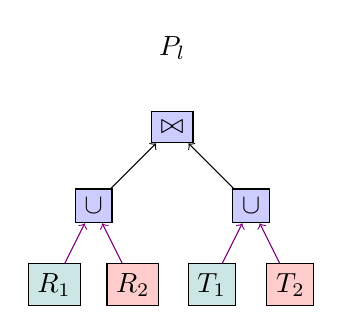
\begin{tikzpicture}
                        \node at (0, 0) {$P_l$};
                        \node[draw, fill=blue!20] (j) at (0, -1) {$\bowtie$};
                        \node[draw, fill=blue!20] (u1) at (-1, -2) {$\cup$};
                        \node[draw, fill=blue!20] (u2) at (1, -2) {$\cup$};
                        \node[draw, fill=teal!20] (r1) at (-1.5, -3) {$R_1$};
                        \node[draw, fill=red!20] (r2) at (-0.5, -3) {$R_2$};
                        \node[draw, fill=teal!20] (t1) at (0.5, -3) {$T_1$};
                        \node[draw, fill=red!20] (t2) at (1.5, -3) {$T_2$};

                        \draw
                        (r1) edge[violet, ->] (u1)
                        (r2) edge[violet, ->] (u1)
                        (t1) edge[violet, ->] (u2)
                        (t2) edge[violet, ->] (u2)
                        (u1) edge[->] (j)
                        (u2) edge[->] (j);
                    \end{tikzpicture}
                    \hfill
                    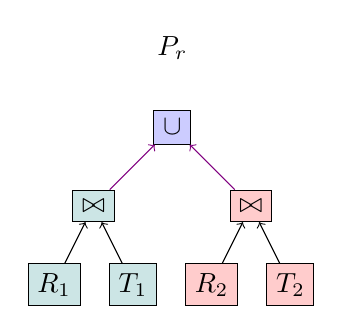
\begin{tikzpicture}
                        \node at (0, 0) {$P_r$};
                        \node[draw, fill=blue!20] (u) at (0, -1) {$\cup$};
                        \node[draw, fill=teal!20] (j1) at (-1, -2) {$\bowtie$};
                        \node[draw, fill=red!20] (j2) at (1, -2) {$\bowtie$};
                        \node[draw, fill=teal!20] (r1) at (-1.5, -3) {$R_1$};
                        \node[draw, fill=teal!20] (t1) at (-0.5, -3) {$T_1$};
                        \node[draw, fill=red!20] (r2) at (0.5, -3) {$R_2$};
                        \node[draw, fill=red!20] (t2) at (1.5, -3) {$T_2$};

                        \draw
                        (r1) edge[->] (j1)
                        (t1) edge[->] (j1)
                        (r2) edge[->] (j2)
                        (t2) edge[->] (j2)
                        (j1) edge[violet, ->] (u)
                        (j2) edge[violet, ->] (u);
                    \end{tikzpicture}
                    \hfill \phantom{}
                \end{center}
                This gives us the following query costs;
                \begin{align*}
                    NDB(P_l) & = |R| \cdot \text{RowSize}(R) + |T| \cdot \text{RowSize}(T) \\
                    NDB(P_r) & = |R \bowtie T| \cdot \text{RowSize}(R \bowtie T)
                \end{align*}
            \subsubsection*{Intersite Communication}
                If two relations are horizontally fragment, such that we have;
                $$R = R_1 \cup \dots \cup R_i, S = S_1 \cup \dots \cup S_i$$
                To perform a join on $R$ and $S$ will require intersite communication;
                $$R \bowtie S = (R_1 \bowtie (S_1 \cup \dots \cup S_i)) \cup \dots (R_i \bowtie (S_1 \cup \dots \cup S_i))$$
                However, if derived horizontal fragmentation had been used, such that we have $R_i = R \ltimes S_i$, we require \textbf{no intersite communication};
                $$R \bowtie S \equiv (R_1 \bowtie S_1) \cup \dots \cup (R_i \bowtie S_i)$$
                As such, the design of a DDB schema should use derived horizontal fragmentation to avoid intersite communication for commonly used joins.
        \subsection*{Topic 8 - Serialisability and Recoverability}
            This lecture starts with ACID properties of transactions, which I won't go over again.
            \subsubsection*{Histories}
                Note that we will denote read operations on objects as $r_n[o_j]$ and writes as $w_n[o_j]$.
                At the end of the transaction, it will either result in $c_n$ for commitment, or $a_n$ if the transaction is aborted (undo all parts of the transaction).
                If $b_n$ is at the start, it denotes the start of a transaction (not always given).
                For example;
                \begin{center}
                    \begin{minipage}[t]{0.485\textwidth}
                        \vspace{-\baselineskip}
                        \begin{lstlisting}
                            BEGIN TRANSACTION
                              UPDATE branch
                              SET    cash = cash - 10000.00
                              WHERE  sortcode = 56

                              UPDATE branch
                              SET    cash = cash + 10000.00
                              WHERE  sortcode = 34
                            COMMIT TRANSACTION
                        \end{lstlisting}
                    \end{minipage}
                    \hfill
                    \begin{minipage}[t]{0.485\textwidth}
                        Would be converted into the following ($H_1 =$)
                        \begin{itemize}
                            \itemsep0em
                            \item $r_1[b_{56}], ~cash=94340.45~$
                            \item $w_1[b_{56}], ~cash=84340.45~$
                            \item $r_1[b_{34}], ~cash=8900.67~$
                            \item $w_1[b_{34}], ~cash=18900.67~$
                            \item $c_1$
                        \end{itemize}
                    \end{minipage}
                \end{center}
                Note that the same pattern of transaction code will give the same pattern of operations;
                \begin{center}
                    \begin{minipage}[t]{0.485\textwidth}
                        \vspace{-\baselineskip}
                        \begin{lstlisting}
                            BEGIN TRANSACTION
                              UPDATE branch
                              SET    cash = cash - 2000.00
                              WHERE  sortcode = 34

                              UPDATE branch
                              SET    cash = cash + 2000.00
                              WHERE  sortcode = 67
                            COMMIT TRANSACTION
                        \end{lstlisting}
                    \end{minipage}
                    \hfill
                    \begin{minipage}[t]{0.485\textwidth}
                        Would be converted into the following ($H_2 =$)
                        \begin{itemize}
                            \itemsep0em
                            \item $r_2[b_{34}], ~cash=18900.67~$
                            \item $w_2[b_{34}], ~cash=16900.67~$
                            \item $r_2[b_{67}], ~cash=34005.00~$
                            \item $w_2[b_{67}], ~cash=36005.00~$
                            \item $c_2$
                        \end{itemize}
                    \end{minipage}
                \end{center}
                In a concurrent execution, the order of operations within each history is preserved, however interleaving can occur.
                \medskip

                \textbf{Serialisability} means that a concurrent execution of transaction should have the same end result as a serial execution of the same transactions.
                \textbf{Recoverability} means that no transaction commits depending on data that has been produced by another transaction which hasn't yet committed.
                The latter can be clarified with an example; if the $b_{34}$ read and write in $H_2$ is done first, before $H_1$, and then $c_2$ happens \textbf{before} $c_1$, we have something that is serialisable and recoverable.
            \subsubsection*{Anomalies}
                We can have a number of anomalies occurring;
                \begin{itemize}
                    \itemsep0em
                    \item \textbf{lost updates}
                        \smallskip

                        If we were to have some sort of execution in the order $r_2[b_{34}], r_1[b_{34}], w_1[b_{34}], w_2[b_{34}]$, notice that the same value is read in for both, and therefore the first write ($w_1[b_{34}]$) will be lost.
                        This is not serialisable, however it is recoverable since neither are reading a result that was changed by the other.
                    \item \textbf{inconsistent analysis}
                        \smallskip

                        This is the example at the start of the lecture, where we take the sum of the balances of the branches, which happens between a transaction (money is removed from one branch but \textbf{not} yet added to another).
                        Note that the order of the commits at the end determine if it is recoverable (if $c_1$ commits first, then it is fine, since the sum transaction depends on the transfer).
                    \item \textbf{dirty reads}
                        \smallskip

                        A dirty read occurs when a transaction reads from data that another transaction has not yet committed.
                        The example given for this is that $w_2[b_{34}]$ occurs before $r_1[b_{34}]$, and then $c_1$ occurs (after the write) and $a_2$ happens at the end, this is serialisable, but not recoverable.
                    \item \textbf{dirty write}
                        \smallskip

                        In this example, an updates are done on the same field on multiple accounts.
                        If there is an interleaving between these two transactions, it results in some updates being applied from the first transaction and some being applied from the second.
                    \item \textbf{phantom reads}
                        \smallskip

                        The example given for this is an update on a rule (~rate < 5.5~), and then a new row gets inserted which would've satisfied that, which is then updated by another update in the first transaction.
                    \item \textbf{write skew}
                        \smallskip

                        This performs two different write operations based on overlapping information, where it could not have been performed if it were executed in a serial order.
                \end{itemize}
                We can summarise it as follows, where $e_i$ means either $c_i$ or $a_i$ occurs, and $op_a \prec op_b$ means that $op_a$ occurs before $op_b$ in a history;
                \begin{center}
                    \begin{tabular}{ll}
                        anomaly & pattern \\
                        \hline
                        dirty write & $w_1[o] \prec w_2[o] \prec e_1$ \\
                        dirty read & $w_1[o] \prec r_2[o] \prec e_1$ \\
                        inconsistent analysis & $r_1[o_a] \prec w_2[o_a], w_2[o_b] \prec r_1[o_b]$ \\
                        lost update & $r_1[o] \prec w_2[o] \prec w_1[o]$
                    \end{tabular}
                \end{center}
            \subsubsection*{Serialisability}
                If we notice in some history ($H$) of anomalies a transaction that has been aborted, we can omit it and only look at the \textbf{committed projection} ($C(H)$).
                \medskip

                A \textbf{conflict} occurs when there is an interaction between two transaction.
                The cases are when $r_x[o]$ and $w_y[o]$ are both in $H$, with $x \neq y$, or both $w_x[o]$ and $w_y[o]$ are in $H$, with $x \neq y$ again.
                \medskip

                We define two histories $H_i$ and $H_j$ to be \textbf{conflict equivalent} ($H_i \equiv_{CE} H_j$) if they contain the same set of operations and order conflicts (of non-aborted transactions) in the same way.
                A history $H$ is \textbf{conflict serialisable} if $C(H) \equiv_{CE}$ a serial history.
                \medskip

                We can draw a \textbf{serialisation graph} $SG(H)$ which contains a node for each transaction in $H$, and an edge $T_i \to T_j$ if there exist some object $o$, for which a conflict $rw_i[o] \to rw_j[o]$ exists in $H$.
                If this graph is acyclic, then $H$ is conflict serialisable.
                For example, consider the following history;
                $$H_{cp} = \red{r_1[b_{56}]}, \teal{r_2[b_{34}]}, \teal{w_2[b_{34}]}, \red{w_1[b_{56}]}, \violet{r_4[b_{56}]}, \red{r_1[b_{34}]}, \red{w_1[b_{34}]}, \red{c_1}, \violet{r_4[b_{34}]}, \teal{r_2[b_{67}]}, \teal{w_2[b_{67}]}, \teal{c_2}, \violet{r_4[b_{67}]}, \violet{c_4}$$
                From this, we obtain the following conflicts;
                \begin{enumerate}[1.]
                    \itemsep0em
                    \item $\teal{w_2[b_{34}]} \to \red{r_1[b_{34}]}$
                    \item $\red{w_1[b_{56}]} \to \violet{r_4[b_{56}]}$
                    \item $\red{w_1[b_{34}]} \to \violet{r_4[b_{34}]}$
                    \item $\teal{w_2[b_{67}]} \to \violet{r_4[b_{67}]}$
                \end{enumerate}
                Using this, we can draw the following acyclic graph, $S(H_{cp})$, hence we can say that $H_{cp}$ is conflict serialisable, with an order $T_2, T_1, T_4$;
                \begin{center}
                    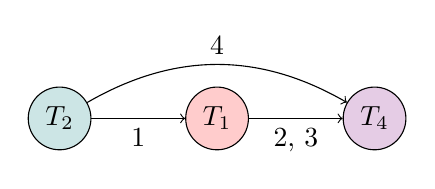
\begin{tikzpicture}[y=1.5cm]
                        \node[circle, draw, fill=teal!20] (t2) at (0, 0) {$T_2$};
                        \node[circle, draw, fill=red!20] (t1) at (2, 0) {$T_1$};
                        \node[circle, draw, fill=violet!20] (t4) at (4, 0) {$T_4$};

                        \draw
                        (t2) edge[->, below] node{1} (t1)
                        (t1) edge[->, below] node{2, 3} (t4)
                        (t2) edge[->, above, bend left=30] node{4} (t4);
                    \end{tikzpicture}
                \end{center}
            \subsubsection*{Recoverability}
                Serialisability is necessary for isolation and consistency of committed transaction, whereas recoverability is necessary for isolation and consistency when there are also aborted transactions.
                Some categories of histories are as follows;
                \begin{itemize}
                    \itemsep0em
                    \item \textbf{recoverable execution (RC)}
                        \subitem a history $H$ has no transaction committing before another transaction from which it read
                    \item \textbf{execution avoiding cascading aborts (ACA)}
                        \subitem does not read from a non-committed transaction (does not allow any dirty reads to occur)
                    \item \textbf{strict execution (ST)}
                        \subitem does not read from a non-committed transaction, nor write over a non-committed transaction (no dirty reads nor writes)
                \end{itemize}
                There's some examples in the lecture slides, but they're quite tedious to copy out.
        \subsection*{Topic 9 - Concurrency Control}
            The main approach we cover in this course is \textbf{two-phase locking (2PL)}, which directly implements the ideas of conflict previously mentioned.
            This approach uses locks to prevent problematic patterns.
            \medskip

            Other approaches include time-stamping / version control, which only reads or writes objects with earlier timestamps, and aborts any changes when the object has a newer timestamp.
            Another approach is optimistic concurrency control which does nothing until the commit, at which point the history is inspected for problems.
            \subsubsection*{2PL Protocol}
                The protocol is as follows;
                \begin{enumerate}[1.]
                    \itemsep0em
                    \item read locks $rl[o], \dots, r[o], \dots, ru[o]$
                    \item write locks $wl[o], \dots, w[o], \dots, wu[o]$
                    \item has two phases
                        \begin{enumerate}[i.]
                            \itemsep0em
                            \item growing phase
                            \item shrinking phase
                        \end{enumerate}
                        Note that more locks cannot be acquired during the shrinking phase.
                    \item refuse $rl_i[o]$ if $wl_j[o]$ is already held, and refuse $wl_i[o]$ if $rl_j[o]$ \textbf{or} $wl_j[o]$ are already held
                    \item if $rl_i[o]$ or $wl_i[o]$ is refused, then delay $T_i$
                \end{enumerate}
                2PL works because we can re-time the history to have all operations occurring during the maximum lock period.
                This is CSR since all conflicts must be prevented during the maximum lock period.
                \medskip

                Revisiting the phantom read anomaly, naive 2PL has an issue with inserting.
                Since no lock would be acquired for the new object (from the insert), the insert is able to happen without any refusal.
                The lock should've been done on the predicate, rather than the individual objects.
                There are some solutions;
                \begin{itemize}
                    \itemsep0em
                    \item \textbf{table lock}
                        \smallskip

                        The problem with a phantom read is due to the changing the data which matches a query, and here we acquire a read lock when performing a `scan' of the table.
                        This can produce needless conflicts, however it can be quite efficient of large parts of the table are being updated.
                        As such, it would lock the entire table, for example $wl_7[a]$, rather than $wl_7[a_{101}]$ and $wl_7[a_{119}]$.
                    \item \textbf{predicate locking / range locking}
                        \smallskip

                        As the name implies, this locks on a predicate, which is more difficult to implement than the table lock.
                        In this example, it would first acquire a read lock on the predicate, and then acquire individual write locks on each of the rows.
                \end{itemize}
            \subsubsection*{Scheduling}
                An \textbf{aggressive scheduler} delays taking locks as long as possible (only acquires the relevant lock before an operation).
                This is simple to implement, and maximises concurrency, however it may suffer delays later on.
                For example, if we needed to acquire a lock right at the end of our transaction (before all the other locks are released), but something else is holding it, any transaction waiting for the locks we're currently holding will also be delayed.
                \medskip

                A \textbf{strict locking} variation prevents write locks from being released before the transaction ends (however read locks can be).
                This allows for deadlocks.
                Since write locks cannot be released, dirt reads / writes are avoided, and it is recoverable.

                On the other hand a \textbf{strong strict locking} variation prevents any locks from being released before the transaction ends.
                This is simple to implement, and is also suitable for distributed transactions.
                \medskip

                On the other hand, a \textbf{conservative scheduler} takes locks as soon as possible, and then releases them as it finishes.
                This removes the risk of delays later on, however the transaction may refuse to start (since it relies on all the locks being available).
                This prevents deadlock, but the problem is to figure out when to release locks.
                It is also not recoverable.
                \medskip

                We can detect deadlocks with a WFG (waits-for graph).
                If a cycle is present in the graph, that means the database is in a deadlock state, and something must be aborted.
            \subsubsection*{Anomalies Summarised}
                Using the same notation as before, we now have the following;
                \begin{center}
                    \begin{tabular}{lll}
                        anomaly & pattern & prevented by \\
                        \hline
                        dirty write & $w_1[o] \prec w_2[o], w_2[o] \prec e_1$ & strict 2PL \\
                        dirty read & $w_1[o] \prec r_2[o], r_2[o] \prec e_1$ &  strict 2PL \\
                        inconsistent analysis & $r_1[o_a] \prec w_2[o_a], w_2[o_b] \prec r_1[o_b]$ & 2PL \\
                        lost update & $r_1[o] \prec w_2[o], \prec w_2[o] \prec w_1[o]$ & 2PL \\
                        simple write skew & $r_1[o_a] \prec w_2[o_b], r_1[o_b] \prec w_2[o_a]$ & 2PL \\
                        write skew & $r_1[P_1] \prec w_2[x \in P_2], r_2[P_2] \prec w_1[y \in P_1]$ & 2PL (with pred. locks) \\
                        phantom read & $r_1[P_1] \prec w_2[x \in P_1], w_2[y \in P_2] \prec r_1[P_2]$ & 2PL (with pred. locks)
                    \end{tabular}
                \end{center}
            \subsubsection*{Isolation Levels}
                Note that we don't \textbf{always} need ACID properties.
                If we are doing something with an approximate result, such as obtaining an estimate, or some sort of overview, we can execute these transactions at a lower level of concurrency control.
                \begin{itemize}
                    \itemsep0em
                    \item ~READ UNCOMMITTED~
                        \smallskip

                        This is the weakest level, which only prevents dirty writes.
                    \item ~READ COMMITTED~
                        \smallskip

                        Prevents dirty reads and writes, which allows transactions to only read committed data.
                        This is recoverable, but can still suffer inconsistent analysis.
                    \item ~SNAPSHOT~
                        \smallskip

                        Allows transactions to see a view of the data at the start of the transaction, and write all data at the end of the transaction.
                        This prevents every anomaly, other than write skew.
                    \item ~REPEATABLE READ~
                        \smallskip

                        This allows inserts to tables which are already read, and prevents everything other than phantom reads.
                \end{itemize}
        \subsection*{Topic 10 - Distributed Transactions}
            \subsubsection*{Distributed 2PL}
                With 2PL, we have the issue of synchronising the two phases across the different sites.
                Adopting a strong strict locking approach will amount to coordinating committment of transactions, which is the standard approach.
                If we're fragmenting data, we simply fragment the lock to the site where the relavent fragment of the data is present.
                Replication means that we need to, to some extent, copy the locks across the different sites.
            \subsubsection*{WFG}
                We can convert a centralised WFG to sub-transactions by introducing bidirectional spawning edges;
                \begin{center}
                    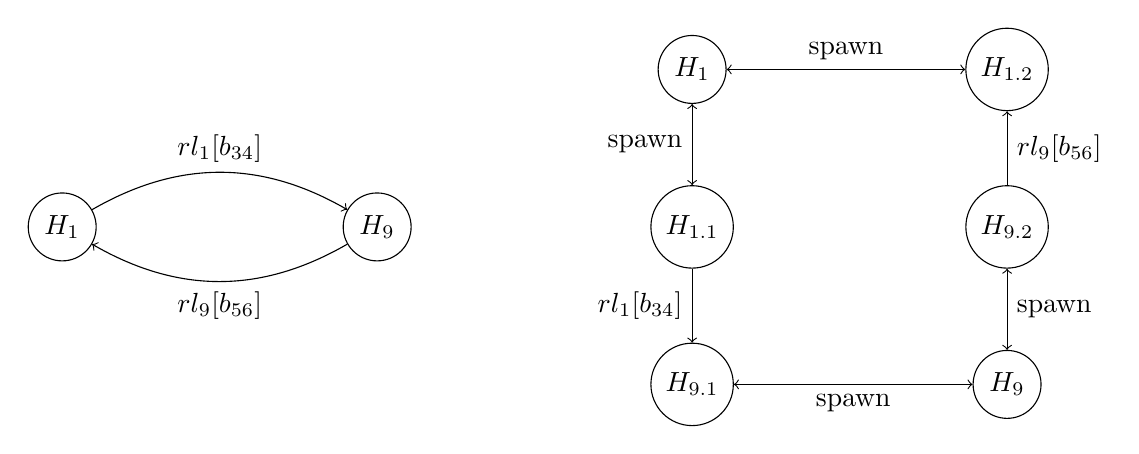
\begin{tikzpicture}[y=0.5cm]
                        \node[draw, circle] (h1a) at (0, 0) {$H_1$};
                        \node[draw, circle] (h9a) at (4, 0) {$H_9$};
                        \draw
                        (h1a) edge[->, above, bend left=30] node{$rl_1[b_{34}]$} (h9a)
                        (h9a) edge[->, below, bend left=30] node{$rl_9[b_{56}]$} (h1a);

                        \node[draw, circle] (h1b) at (8, 4) {$H_1$};
                        \node[draw, circle] (h12) at (12, 4) {$H_{1.2}$};
                        \node[draw, circle] (h11) at (8, 0) {$H_{1.1}$};
                        \node[draw, circle] (h92) at (12, 0) {$H_{9.2}$};
                        \node[draw, circle] (h91) at (8, -4) {$H_{9.1}$};
                        \node[draw, circle] (h9b) at (12, -4) {$H_9$};

                        \draw
                        (h1b) edge[<->, left] node{spawn} (h11)
                        (h1b) edge[<->, above] node{spawn} (h12)
                        (h9b) edge[<->, below] node{spawn} (h91)
                        (h9b) edge[<->, right] node{spawn} (h92)
                        (h11) edge[->, left] node{$rl_1[b_{34}]$} (h91)
                        (h92) edge[->, right] node{$rl_9[b_{56}]$} (h12);
                    \end{tikzpicture}
                \end{center}
                When a local cycle is detected, the remote WFG is fetched and recombined to see if a cycle has been formed in the global WFG.
                If that the case, one of the transactions are aborted.
                Deadlock might have ocurred once a cycle has appeared at any node executing a distributed transaction.
            \subsubsection*{Global 2PL and 2PC}
                The incorrect approach for performing 2PL globally would be to execute 2PL at each site.
                The correct approach would be to adopt strong strict locking at each site, and then the transactions can be ended with an global atomic commit.
                \medskip

                In two-phase commit (2PC), we have the following (note that the coordinator could also operate from one of the servers, doesn't have to be a separate host);
                \begin{center}
                    \begin{tabular}{lll}
                        service element & source & semantics \\
                        \hline
                        ~C-PREPARE~ & coordinator & get ready to commit \\
                        ~C-READY~ & server & ready to commit \\
                        ~C-REFUSE~ & server & not ready to commit \\
                        ~C-COMMIT~ & coordinator & commit the transaction \\
                        ~C-ROLLBACK~ & server & rollback the transaction \\
                        ~C-RESTART~ & either & try to return to start of transaction
                    \end{tabular}
                \end{center}
                If either of the servers sends a ~C-REFUSE.request~ (instead of ~C-READY.request~) after a ~C-PREPARE.request~ from the server, a ~C-ROLLBACK.request~ is sent from the coordinator to both the servers, and a ~C-ROLLBACK.response~ is sent from the server \textbf{not} requesting the refusal.
                On the other hand, if both send ~C-READY~, a ~C-COMMIT~ is sent from the coordinator.
                \medskip

                If one of the servers crashes however, it can lead to blocking, since the non-crashed server will not know whether to commit or to abort.
            \subsubsection*{Sending Locks}
                If we have fragmented data, the locks $wl_x[o]$ or $rl_x[o]$ must be sent to the host containing $o$.
                On the other hand, if we have replicated data, $w_x[o]$ must be sent to all hosts containing $o$.
                Similarly we can send send $r_w[o]$ to any host containing $o$.
                \medskip

                As long as we send locks to the \textbf{majority} of sites, we will detect a write-write conflict.
                Therefore the number of locks we send;
                $$j \geq \ceil{\frac{n + 1}{2}}$$
                On the other hand, to detect a read-write conflict, the number of locks we send, where $k$ is the number of read locks, and $j$ the number of write locks;
                $$j \geq n - k + 1$$
\end{document}